%%%%%%%%%%%%%%%%%%%%%%%%%%%%%%%%%%%%%%%%%
% Masters/Doctoral Thesis 
% LaTeX Template
% Version 2.5 (27/8/17)
%
% This template was downloaded from:
% http://www.LaTeXTemplates.com
%
% Version 2.x major modifications by:
% Vel (vel@latextemplates.com)
%
% This template is based on a template by:
% Steve Gunn (http://users.ecs.soton.ac.uk/srg/softwaretools/document/templates/)
% Sunil Patel (http://www.sunilpatel.co.uk/thesis-template/)
%
% Template license:
% CC BY-NC-SA 3.0 (http://creativecommons.org/licenses/by-nc-sa/3.0/)
%
%%%%%%%%%%%%%%%%%%%%%%%%%%%%%%%%%%%%%%%%%

%----------------------------------------------------------------------------------------
%	PACKAGES AND OTHER DOCUMENT CONFIGURATIONS
%----------------------------------------------------------------------------------------

\documentclass[
11pt, % The default document font size, options: 10pt, 11pt, 12pt
%oneside, % Two side (alternating margins) for binding by default, uncomment to switch to one side
english, % ngerman for German
singlespacing, % Single line spacing, alternatives: onehalfspacing or doublespacing
%draft, % Uncomment to enable draft mode (no pictures, no links, overfull hboxes indicated)
%nolistspacing, % If the document is onehalfspacing or doublespacing, uncomment this to set spacing in lists to single
%liststotoc, % Uncomment to add the list of figures/tables/etc to the table of contents
%toctotoc, % Uncomment to add the main table of contents to the table of contents
%parskip, % Uncomment to add space between paragraphs
%nohyperref, % Uncomment to not load the hyperref package
headsepline, % Uncomment to get a line under the header
%chapterinoneline, % Uncomment to place the chapter title next to the number on one line
%consistentlayout, % Uncomment to change the layout of the declaration, abstract and acknowledgements pages to match the default layout
]{MastersDoctoralThesis} % The class file specifying the document structure

\usepackage[utf8]{inputenc} % Required for inputting international characters
\usepackage[T1]{fontenc} % Output font encoding for international characters

\usepackage{mathpazo} % Use the Palatino font by default

\usepackage[backend=bibtex,style=numeric,natbib=true, sorting=none]{biblatex} % Use the bibtex backend with the authoryear citation style (which resembles APA)

\addbibresource{refs.bib} % The filename of the bibliography

\usepackage[autostyle=true]{csquotes} % Required to generate language-dependent quotes in the bibliography

\usepackage{bm} % to use $\boldsymbol{}$
\usepackage{amsmath}
\usepackage{amssymb}
\usepackage{verbatim} % to use the \begin{comment} block
\usepackage{subfigure}

\usepackage{tikz}
\usetikzlibrary{intersections}
\usetikzlibrary{angles, patterns, calc, quotes}%calc,patterns,angles,quotes}

\newcommand\encircle[1]{%
	\tikz[baseline=(X.base)] 
	\node (X) [draw, shape=circle, inner sep=0] {\strut #1};} %to encirle letters

%----------------------------------------------------------------------------------------
%	MARGIN SETTINGS
%----------------------------------------------------------------------------------------

\geometry{
	paper=a4paper, % Change to letterpaper for US letter
	inner=2.5cm, % Inner margin
	outer=3.8cm, % Outer margin
	bindingoffset=.5cm, % Binding offset
	top=1.5cm, % Top margin
	bottom=1.5cm, % Bottom margin
	%showframe, % Uncomment to show how the type block is set on the page
}

%----------------------------------------------------------------------------------------
%	THESIS INFORMATION
%----------------------------------------------------------------------------------------

\thesistitle{Measurement of Higgs Boson CP Properties} % Your thesis title, this is used in the title and abstract, print it elsewhere with \ttitle
\supervisor{Prof. Achim \textsc{Stahl} \\ Prof. Oliver \textsc{Pooth}} % Your supervisor's name, this is used in the title page, print it elsewhere with \supname
\examiner{} % Your examiner's name, this is not currently used anywhere in the template, print it elsewhere with \examname
\degree{Bachelor of Science} % Your degree name, this is used in the title page and abstract, print it elsewhere with \degreename
\author{Mate Zoltan \textsc{Farkas}} % Your name, this is used in the title page and abstract, print it elsewhere with \authorname
\addresses{} % Your address, this is not currently used anywhere in the template, print it elsewhere with \addressname

\subject{Physics} % Your subject area, this is not currently used anywhere in the template, print it elsewhere with \subjectname
\keywords{} % Keywords for your thesis, this is not currently used anywhere in the template, print it elsewhere with \keywordnames
\university{\href{http://www.rwth-aachen.de}{RWTH Aachen University}} % Your university's name and URL, this is used in the title page and abstract, print it elsewhere with \univname
\department{\href{http://www.physik.rwth-aachen.de/cms/~mya/Physik/?lidx=1}{Department of Physics}} % Your department's name and URL, this is used in the title page and abstract, print it elsewhere with \deptname
\group{\href{http://www.institut3b.physik.rwth-aachen.de/cms/~fslr/ParticlePhysics3B/?lidx=1}{III. Physics Institute B}} % Your research group's name and URL, this is used in the title page, print it elsewhere with \groupname
\faculty{\href{http://www.physik.rwth-aachen.de/cms/~mya/Physik/?lidx=1}{Department of Physics}} % Your faculty's name and URL, this is used in the title page and abstract, print it elsewhere with \facname

\AtBeginDocument{
\hypersetup{pdftitle=\ttitle} % Set the PDF's title to your title
\hypersetup{pdfauthor=\authorname} % Set the PDF's author to your name
\hypersetup{pdfkeywords=\keywordnames} % Set the PDF's keywords to your keywords
\hypersetup{hidelinks}
}

\begin{document}

%\frontmatter % Use roman page numbering style (i, ii, iii, iv...) for the pre-content pages

\pagestyle{plain} % Default to the plain heading style until the thesis style is called for the body content

%----------------------------------------------------------------------------------------
%	TITLE PAGE
%----------------------------------------------------------------------------------------

\begin{titlepage}
\begin{center}

\vspace*{.06\textheight}
{\scshape\LARGE \univname\par}\vspace{1.5cm} % University name
\textsc{\Large Bachelor Thesis}\\[0.5cm] % Thesis type

\HRule \\[0.4cm] % Horizontal line
{\huge \bfseries \ttitle\par}\vspace{0.4cm} % Thesis title
\HRule \\[1.5cm] % Horizontal line
 
\begin{minipage}[t]{0.4\textwidth}
\begin{flushleft} \large
\emph{Author:}\\
\href{}{\authorname} % Author name - remove the \href bracket to remove the link
\end{flushleft}
\end{minipage}
\begin{minipage}[t]{0.4\textwidth}
\begin{flushright} \large
\emph{Supervisor:} \\
\href{}{\supname} % Supervisor name - remove the \href bracket to remove the link  
\end{flushright}
\end{minipage}\\[3cm]
 
\vfill

\large \textit{A thesis submitted in fulfillment of the requirements\\ for the degree of \degreename}\\[0.3cm] % University requirement text
\textit{in the}\\[0.4cm]
\groupname\\\deptname\\[2cm] % Research group name and department name
 
\vfill

{\large \today}\\[4cm] % Date
%\includegraphics{Logo} % University/department logo - uncomment to place it
 
\vfill
\end{center}
\end{titlepage}

%----------------------------------------------------------------------------------------
%	DECLARATION PAGE
%----------------------------------------------------------------------------------------

\begin{comment}

\begin{declaration}
\addchaptertocentry{\authorshipname} % Add the declaration to the table of contents
\noindent I, \authorname, declare that this thesis titled, \enquote{\ttitle} and the work presented in it are my own. I confirm that:

\begin{itemize} 
\item This work was done wholly or mainly while in candidature for a research degree at this University.
\item Where any part of this thesis has previously been submitted for a degree or any other qualification at this University or any other institution, this has been clearly stated.
\item Where I have consulted the published work of others, this is always clearly attributed.
\item Where I have quoted from the work of others, the source is always given. With the exception of such quotations, this thesis is entirely my own work.
\item I have acknowledged all main sources of help.
\item Where the thesis is based on work done by myself jointly with others, I have made clear exactly what was done by others and what I have contributed myself.\\
\end{itemize}
 
\noindent Signed:\\
\rule[0.5em]{25em}{0.5pt} % This prints a line for the signature
 
\noindent Date:\\
\rule[0.5em]{25em}{0.5pt} % This prints a line to write the date
\end{declaration}

\cleardoublepage

\end{comment}
%----------------------------------------------------------------------------------------
%	QUOTATION PAGE
%----------------------------------------------------------------------------------------
\begin{comment}
\vspace*{0.2\textheight}

\noindent\enquote{\itshape Thanks to my solid academic training, today I can write hundreds of words on virtually any topic without possessing a shred of information, which is how I got a good job in journalism.}\bigbreak

\hfill Dave Barry
\end{comment}
%----------------------------------------------------------------------------------------
%	ABSTRACT PAGE
%----------------------------------------------------------------------------------------
\begin{comment}
\begin{abstract}
\addchaptertocentry{\abstractname} % Add the abstract to the table of contents
The Thesis Abstract is written here (and usually kept to just this page). The page is kept centered vertically so can expand into the blank space above the title too\ldots
\end{abstract}
\end{comment}
%----------------------------------------------------------------------------------------
%	ACKNOWLEDGEMENTS
%----------------------------------------------------------------------------------------
\begin{comment}
\begin{acknowledgements}
\addchaptertocentry{\acknowledgementname} % Add the acknowledgements to the table of contents
The acknowledgments and the people to thank go here, don't forget to include your project advisor\ldots
\end{acknowledgements}
\end{comment}
%----------------------------------------------------------------------------------------
%	LIST OF CONTENTS/FIGURES/TABLES PAGES
%----------------------------------------------------------------------------------------

\tableofcontents % Prints the main table of contents

\iffalse
\listoffigures % Prints the list of figures

\listoftables % Prints the list of tables


%----------------------------------------------------------------------------------------
%	ABBREVIATIONS
%----------------------------------------------------------------------------------------
\begin{comment}
\begin{abbreviations}{ll} % Include a list of abbreviations (a table of two columns)

\textbf{LAH} & \textbf{L}ist \textbf{A}bbreviations \textbf{H}ere\\
\textbf{WSF} & \textbf{W}hat (it) \textbf{S}tands \textbf{F}or\\

\end{abbreviations}
\end{comment}
%----------------------------------------------------------------------------------------
%	PHYSICAL CONSTANTS/OTHER DEFINITIONS
%----------------------------------------------------------------------------------------
\begin{comment}
\begin{constants}{lr@{${}={}$}l} % The list of physical constants is a three column table

% The \SI{}{} command is provided by the siunitx package, see its documentation for instructions on how to use it

Speed of Light & $c_{0}$ & \SI{2.99792458e8}{\meter\per\second} (exact)\\
%Constant Name & $Symbol$ & $Constant Value$ with units\\

\end{constants}
\end{comment}
\fi
%----------------------------------------------------------------------------------------
%	SYMBOLS
%----------------------------------------------------------------------------------------
\begin{comment}
\begin{symbols}{lll} % Include a list of Symbols (a three column table)
$\boldsymbol{a}$ & a 3-dimensional vector & \\
$\boldsymbol{M}$ & a matrix & \\
\addlinespace 
$\boldsymbol{x}$ & position vector &  \\
$\boldsymbol{p}$ & the 3-momentum vector & \\
$\boldsymbol{\Sigma}$ & the covariance matrix & \\
$\boldsymbol{v}$ & the position vector to the primary vertex; equivalently $\overrightarrow{OV}$ & \\
$\boldsymbol{d}$ & the IP-vector & \\
%Symbol & Name & Unit \\

\addlinespace % Gap to separate the Roman symbols from the Greek

$\omega$ & angular frequency & \si{\radian} \\

\end{symbols}
\end{comment}
%----------------------------------------------------------------------------------------
%	DEDICATION
%----------------------------------------------------------------------------------------

%\dedicatory{For/Dedicated to/To my\ldots} 



%----------------------------------------------------------------------------------------
%	THESIS CONTENT - CHAPTERS
%----------------------------------------------------------------------------------------

%\mainmatter % Begin numeric (1,2,3...) page numbering

\pagestyle{thesis} % Return the page headers back to the "thesis" style

% Include the chapters of the thesis as separate files from the Chapters folder
% Uncomment the lines as you write the chapters

\chapter{Introduction} % Main chapter title

\label{Chapter1} % For referencing the chapter elsewhere, use \ref{Chapter1} 

The Standard Model (SM) of particle physics has proven to be a successful model to describe the elementary particles and their behaviour. Nevertheless, one had to wait long for the experimental verification of a theory predicting the masses of elementary particles (especially of the weak gauge bosons $W^\pm$ and $Z$) -- the Higgs mechanism.\\
Since the discovery of the Higgs boson in 2012 \parencite{Higgs2,Higgs1}, some of its properties (like the mass, spin and charge) of the newest SM particle have already been measured. Nevertheless, the parity quantum number of the Higgs boson is still an open question, as it has only been accessible in its vector boson couplings. For this purpose, the $H\rightarrow\tau\tau$ decay reactions which were observed during Run 2 of the CMS experiment at CERN at \SI{13}{\tera\electronvolt} energy scale of proton-proton collisions are going to be studied.\\
In these decay reactions, multiple pions and leptons can be produced in the final state. In cases where a $\tau$ decays into a pion or a muon, a decay plane can be constructed using the momentum of the child particle and its impact parameter with respect to the vertex of $\tau$ creation. It can be shown that the angle $\varphi_{CP}^*$ between the $\tau$ decay planes in the zero momentum frame is a CP-sensitive variable  \parencite{Berge_1prong, Berge_CP_Prospects}. Therefore, the correct determination of the impact parameter is of special interest.\\
The goal of this thesis is to find a quantity which helps to improve the event selection of the measurement. In addition, a new helical approach is going to be proposed which can help to improve the reconstruction of the impact parameter vectors.
\chapter{The LHC and the CMS Detector} % Main chapter title

\label{Chapter2} % For referencing the chapter elsewhere, use \ref{Chapter1} 

\section{The Large Hadron Collider}
The Large Hadron Collider (LHC) at CERN is the largest particle accelerator yet built, situated in Geneva, on the French-Swiss border. Since the discovery of the Higgs boson in 2012, it has the main purpose of searching for Beyond Standard Model (BSM) physics.\\
With its circumference of 27 km, it is capable of colliding protons or lead particles up to an energy of 7 TeV, resulting in a total center of mass energy up to 14 TeV. In order to achieve such energy scales, the particles have to go through the injection chain Linac2 -- Proton Synchrotron Booster (PSB) -- Proton Synchrotron (PS) -- Super Proton Synchrotron (SPS) as indicated in Fig.~\ref{fig:lhcstruct}; by the time protons reach the LHC they travel with velocities close to the speed of light (more than 99.99\% of it) \parencite{LHC_Machine}.\\
\begin{figure}[h]
	\centering
	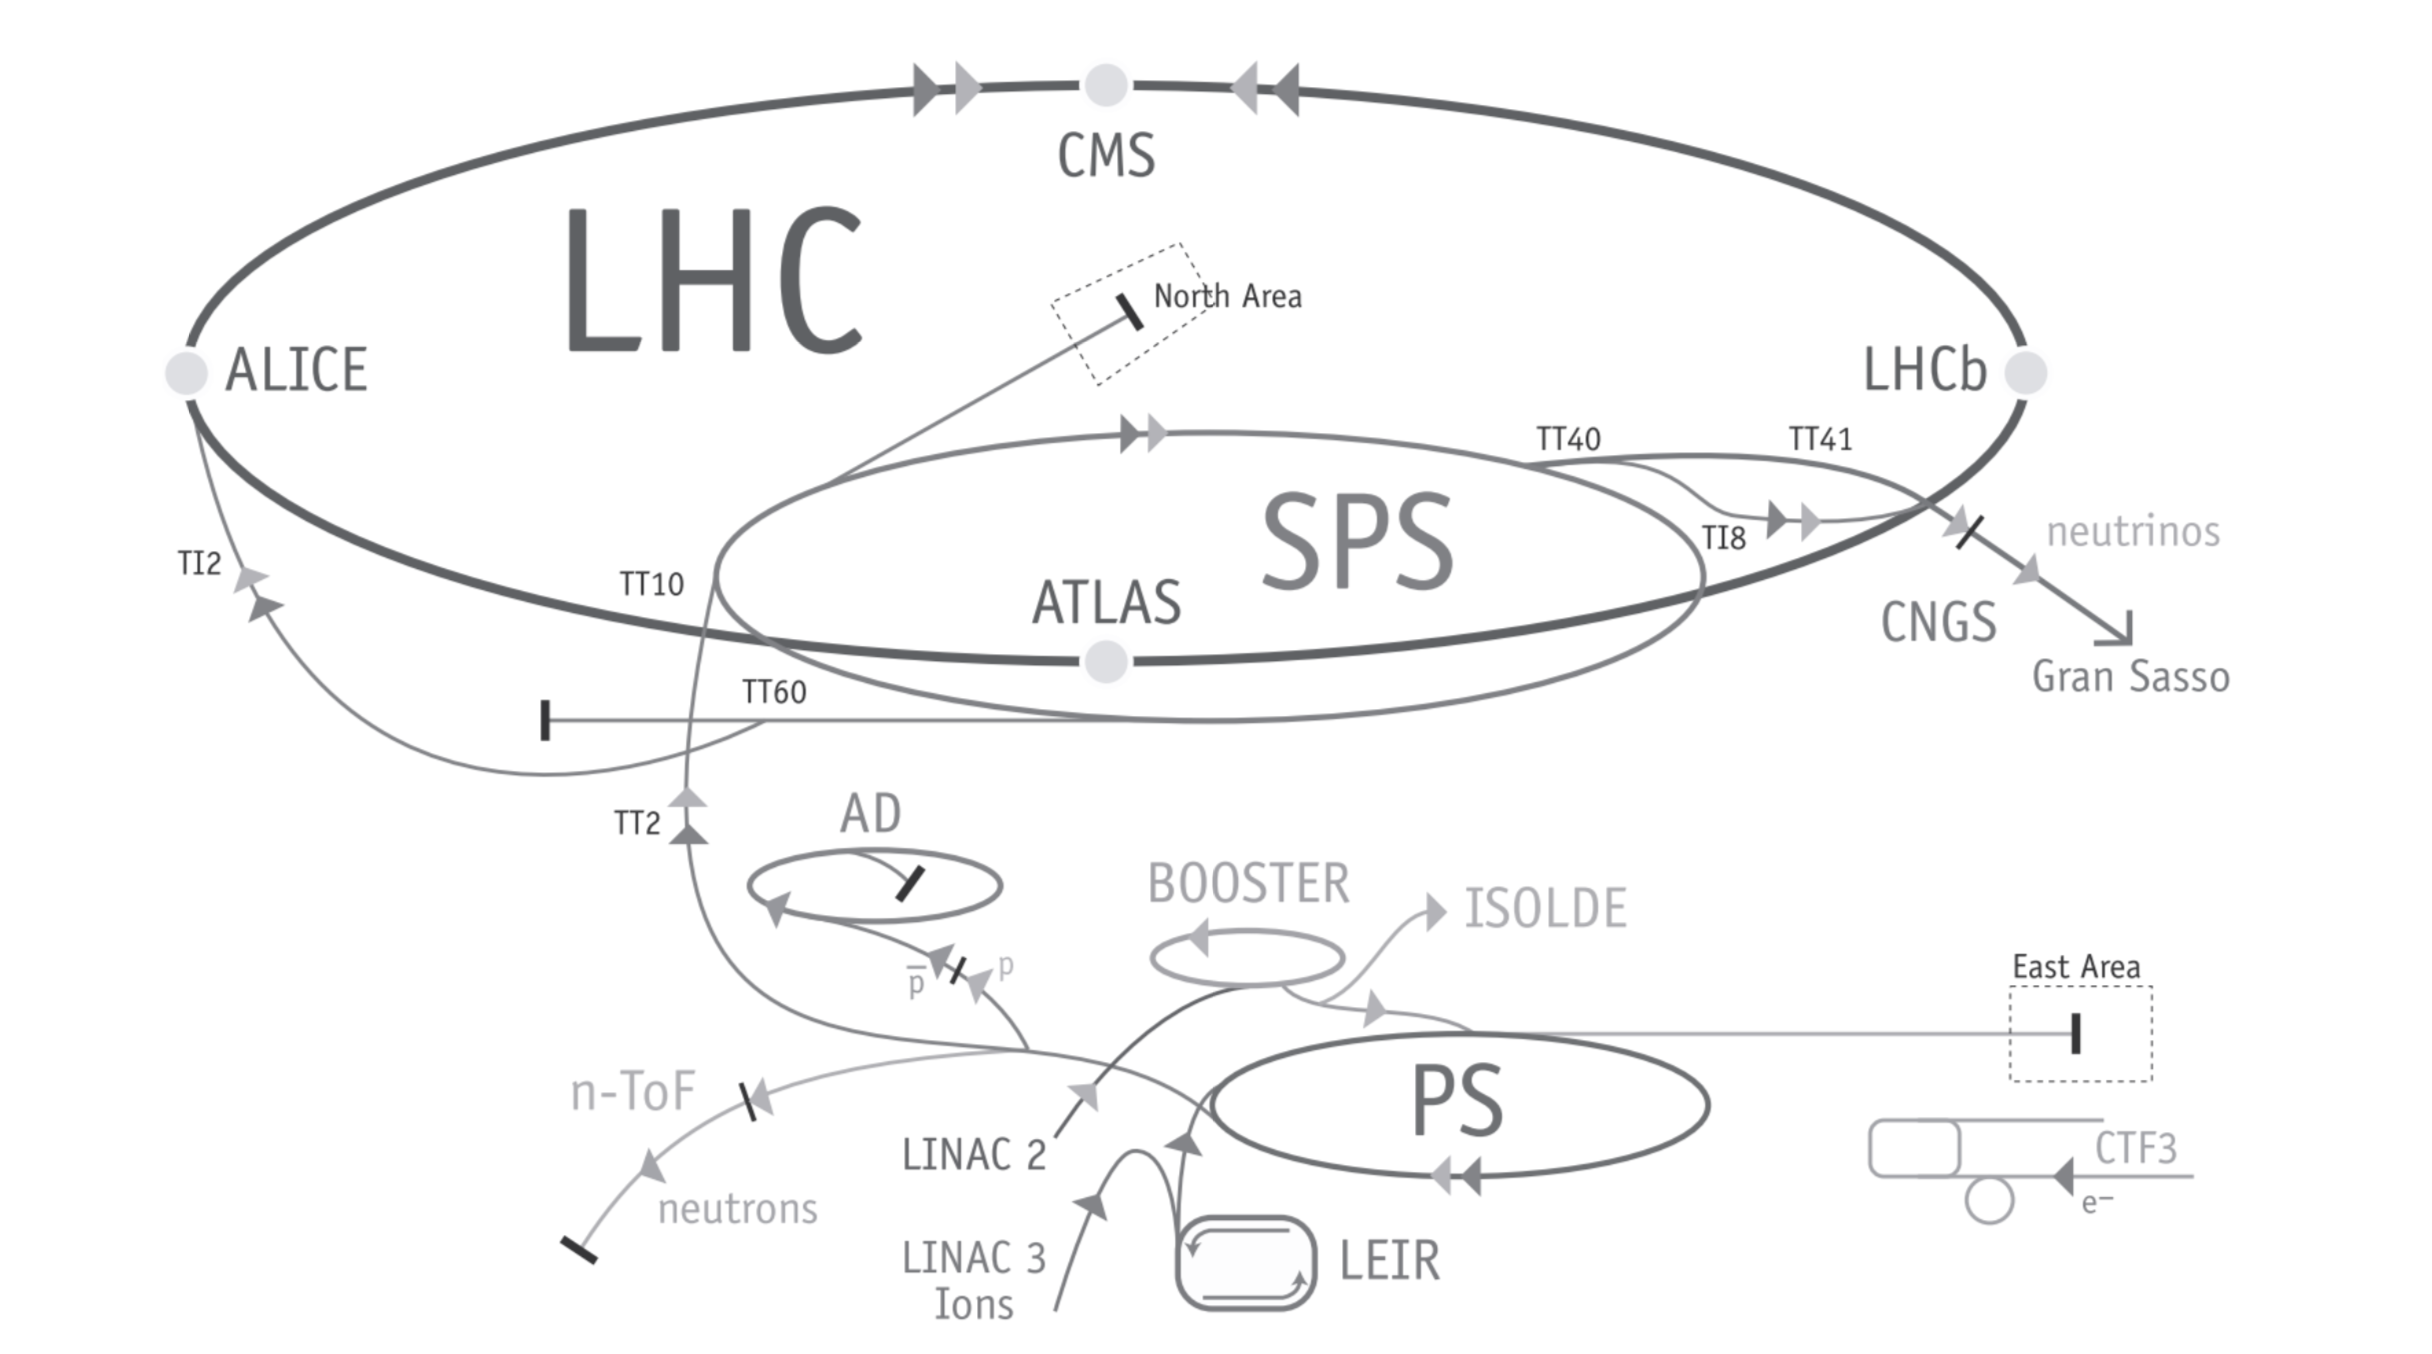
\includegraphics[width=0.7\linewidth]{Figures/LHC_struct}
	\caption{Schematic view of CERN's accelerator structure \parencite{CERN-Guide}}
	\label{fig:lhcstruct}
\end{figure}\\
As one can also see in this figure, there are four primary experiments and detectors situated in the acceleration ring. ALICE is a detector built for heavy ion collisions, LHCb is suitable for measuring top-quarks, ATLAS and CMS are both general purpose detectors. In the following section, the latter is going be introduced briefly, its measurements standing in the focus of this thesis.
\section{The CMS Detector}
The Compact Muon Solenoid (CMS) is a \SI{15}{\meter} wide and \SI{28.7}{\meter} long, onion-like-structured detector, consisting of five main components which are indicated in Fig.~\ref{fig:cms}.
\begin{figure}[h]
	\centering
	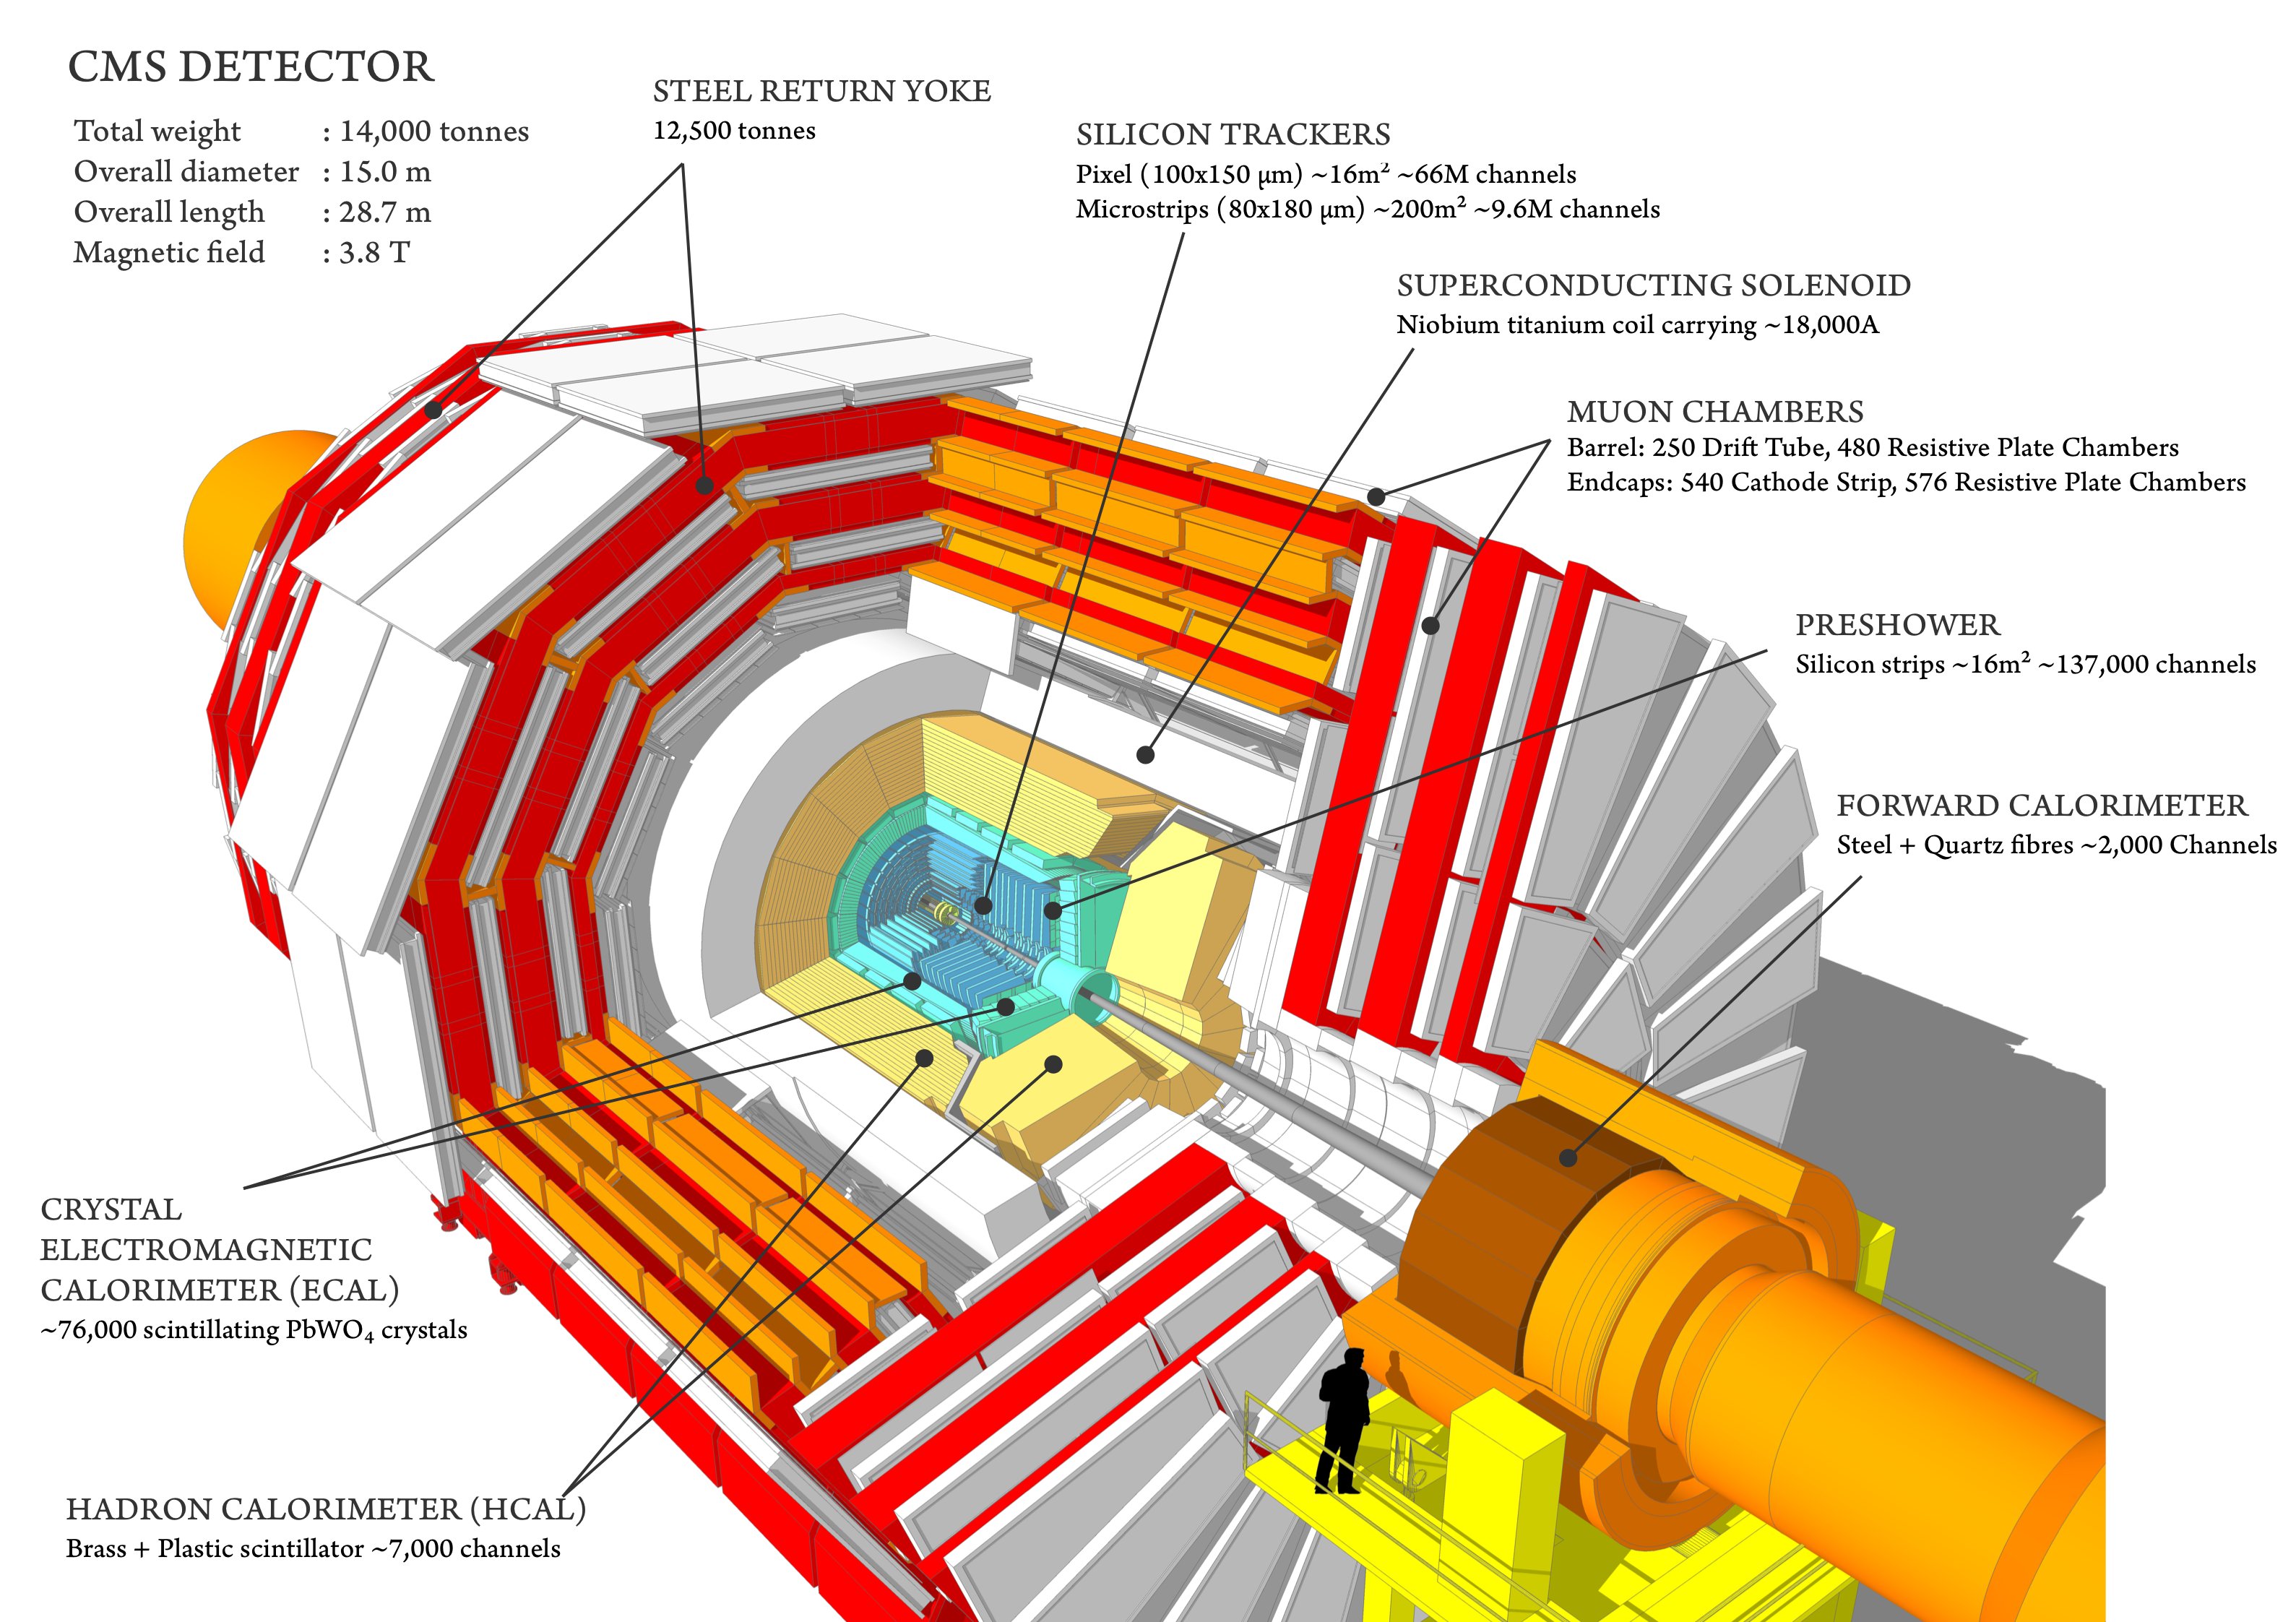
\includegraphics[width=0.9\linewidth]{Figures/CMS}
	\caption{The schematical structure of the CMS detector \parencite{CMS_Detector}}
	\label{fig:cms}
\end{figure}\\
It is built around a huge superconducting solenoid, which can generate a magnetic field of around \SI{3.8}{\tesla}. Its innermost detector component close to the interaction point (the spacial point where the particles collide) is a three layered silicon pixel detector, which with a resolution of 15-\SI{20}{\micro\meter} is capable of reconstructing impact parameters (which have a length of some
\SI{100}{\micro\meter}) and primary vertices. Around it, a silicon strip detector is situated, which can measure the trajectories of particles. Silicon was chosen due to the harsh environment around the collision point to increase the detector lifespan. With an active surface of \SI{200}{\meter\squared}, it is the largest silicon tracker ever built \parencite{CMS_collaboration}.\\
The second component is an electromagnetic calorimeter (ECAL) surrounding the silicon components, providing the measurement of the total energy of electrons and photons. These particles create electromagnetic showers, which can be converted into scintillator light by using lead tungstate crystals $\text{PbWO}_4$. Losing energy, the electrons and photons passing through the detector are eventually stopped in this component, delivering information about their total energy before entrance.\\
Surrounding the ECAL, the third component is the hadronic calorimeter (HCAL), capable of measuring the energy of hadronic jets. Consisting of brass and plastic scintillators, it functions similarly as the ECAL, as hadrons create a cascade of hadronic particles, generating light through scintillation.\\
The CMS detector is structured around the solenoid mentioned above. It is responsible for creating a strong and homogeneous magnetic field inside and outside of the coil in beam direction. This forces the particles to move along helical trajectories, from which through its radius the momentum of these can be measured in the tracking subdetectors.\\
Outside of the coil, the iron return yoke guides the magnetic field having a strength of around \SI{2}{\tesla}. Since muons are not stopped in the ECAL, this enables measuring their momentum for a second time, yielding better resolution and identification.\\
Since this thesis is centered around the measurement of impact parameters, the focus is going to be on the inner part of the detector, where the trajectories of the decay products can be measured.
% Chapter Help

\chapter{Theoretical Background} % Main chapter title

\label{Chapter3} % For referencing the chapter elsewhere, use \ref{Chapter1} 

\section{The IP method}
TODO:
\begin{itemize}
	\item Definiton of IP with plot
\end{itemize}
\label{sec:IP_method}


\chapter{Identification of Events with Well-Reconstructed Decay Planes} % Main chapter title

\label{Chapter4} % For referencing the chapter elsewhere, use \ref{Chapter1} 


The first part of the work presented here is a method to identify the events with well-reconstructed decay planes by applying cuts based on the uncertainty of the impact parameter magnitude. Such cuts have become necessary in order to gain the most information possible in the $\mu\rho$ ($\mu\pi\pi$) final state. For this purpose Monte Carlo (MC) samples are going to be used to study the effects of this cut. In this dataset, the IP is known without uncertainties. Therefore, analysis on the MC-samples is going to be called generator level-study. Reconstruction level indicates the combined analysis of both MC samples and detector effects, the latter giving rise to uncertainties.\\
Mathematically, the problem consists of a 3D vector \textbf{v} (physically the spacial vector of the primary vertex PV), with a given covariance matrix $\boldsymbol{\Sigma}$ encoding the squared uncertainties $\sigma^2_i$ with respect to the PV-vector components and the correlations $\sigma_{ij}$ between them. As for the nature of the processes in the detector, the distribution of these uncertainties can be assumed to be Gaussian, its contour lines describing three-dimensional ellipsoids centred around the primary vertex. This can be easily shown by considering the contour lines of the multivariate normal distribution
\begin{equation}
	G(\boldsymbol{x};\boldsymbol{\Sigma},\boldsymbol{\mu}=\boldsymbol{v}) = \frac{1}{\sqrt{(2\pi)^3\det\boldsymbol{\Sigma}}}\exp{\left[-\frac{1}{2}(\boldsymbol{x}-\boldsymbol{v})^T \boldsymbol{\Sigma}^{-1}(\boldsymbol{x}-\boldsymbol{v}) \right]} = C = const.
\end{equation}
and rearranging all the \textbf{x}-independent terms to the right-hand side of the equation yielding
\begin{equation}
	(\boldsymbol{x}-\boldsymbol{v})^T \boldsymbol{\Sigma}^{-1}(\boldsymbol{x}-\boldsymbol{v}) = -2\cdot\ln\left(C\cdot\sqrt{(2\pi)^3\det\boldsymbol{\Sigma}}\right)=K>0.
\end{equation}
The inequality holds, since both $\boldsymbol{\Sigma}$ and $\boldsymbol{\Sigma^{-1}}$ are positive definite, defining the ellipsoid, similar to its 2D version shown in Fig. \ref{fig:ellipse}.
\begin{figure}[h]
	\centering
	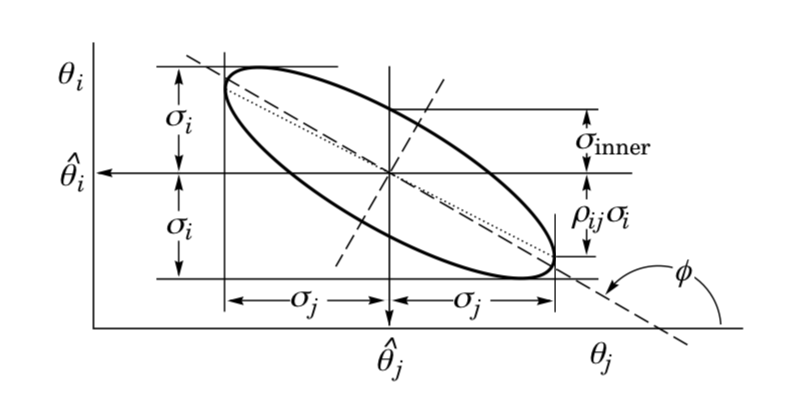
\includegraphics[width=0.7\linewidth]{Figures/ellipsoid}
	\caption{Countour lines of a 2D normal distribution \parencite{PDG_source}}
	\label{fig:ellipse}
\end{figure}\\
In the following, consider the 3-dimensional impact parameter vector \textbf{d} in the reference frame centred around \textbf{v}. Since the direction of \textbf{d} is the physically important quantity in the impact parameter method described in section \ref{sec:IP_method}, it is crucial to exclude the cases where the reconstructed IP points to a different direction then the generated IP vector, giving false results regarding the angle between the $\tau$ decay planes $\varphi^*$. During a real measurement these cases are impossible to identify, therefore one has to apply cuts on the impact parameter based on the uncertainties of \textbf{v}.\\
For this reason, consider the variable $\alpha$, defined as
\begin{equation}
	\alpha = \frac{d}{\sigma_{d}},
\end{equation}
where $d = |\boldsymbol{d}|$, the length of the IP vector. This newly defined variable contains information about the magnitude of the IP from the primary vertex expressed in units of the uncertainty $\sigma_{d}$. In the case where $\alpha = 1$, this means that the endpoints of the IP vector lies on the surface of the uncertainty ellipsoid of the PV. It can be therefore assumed that the chance of a more precisely reconstructed impact parameter direction is higher if the IP vector endpoint is further away from the uncertainty ellipsoid of the primary vertex.\\
Now it remains to determine $\sigma_{d}$. For this, first consider the length of the IP vector $d$
\begin{equation}
	d = \sqrt{d_x^2+d_y^2+d_z^2}
\end{equation}
with which $\sigma_{d}$ can be expressed through the error propagation formula \parencite{Book_error_prop}
\begin{equation}
	\sigma_{d}^2 = \mathbf{J}^T \, \boldsymbol{\Sigma} \, \mathbf{J}
\end{equation}
where \textbf{J} denotes the Jacobian defined as
\begin{equation}
	\mathbf{J} = \nabla d
\end{equation}
with the nabla operator acting on the components of \textbf{d}. This yields however
\begin{equation}
	\nabla d = \partial_i \, d \, \boldsymbol{e}_i = \frac{d_i}{d}\boldsymbol{e}_i = \frac{\boldsymbol{d}}{d} = \boldsymbol{\hat{d}},
\end{equation}
meaning the the uncertainty $\sigma_{d}$ can be written as
\begin{equation}
	\sigma_{d} = \sqrt{\boldsymbol{\hat{d}}^T \, \boldsymbol{\Sigma} \, \boldsymbol{\hat{d}}}
\end{equation}
Now it remains to demonstrate the outputs of such a cut which are summarised in Fig. \ref{fig:lambda_dist}-\ref{fig:lambdacuts_CP}. In Fig. \ref{fig:lambda_dist} the distributions of both $d$ and $\sigma_{d}$ are displayed, which then, define the distribution of the cut parameter $\alpha$ shown in Fig. \ref{fig:IP_magOverLambda_dist}. In Fig. \ref{fig:lambdacuts_angles} (for a CP even scenario in the $\mu\rho$ final state), one can immediately observe the filtering of events where the uncertainty is of the same order as the IP magnitude itself, leading to smaller differences between the generated and reconstructed data. This results in case of $\frac{d}{\sigma_d}\geq7$ in the disappearance of events, where the angle between generated and reconstructed data is greater than 2rad. Similarly promising results can be observed in Fig. \ref{fig:lambdacuts_CP} where one can immediately see the increase in amplitude of the distribution converging to more recognisable $\sin$-like shape.\\
\begin{figure}[h]
	\centering
	\subfigure{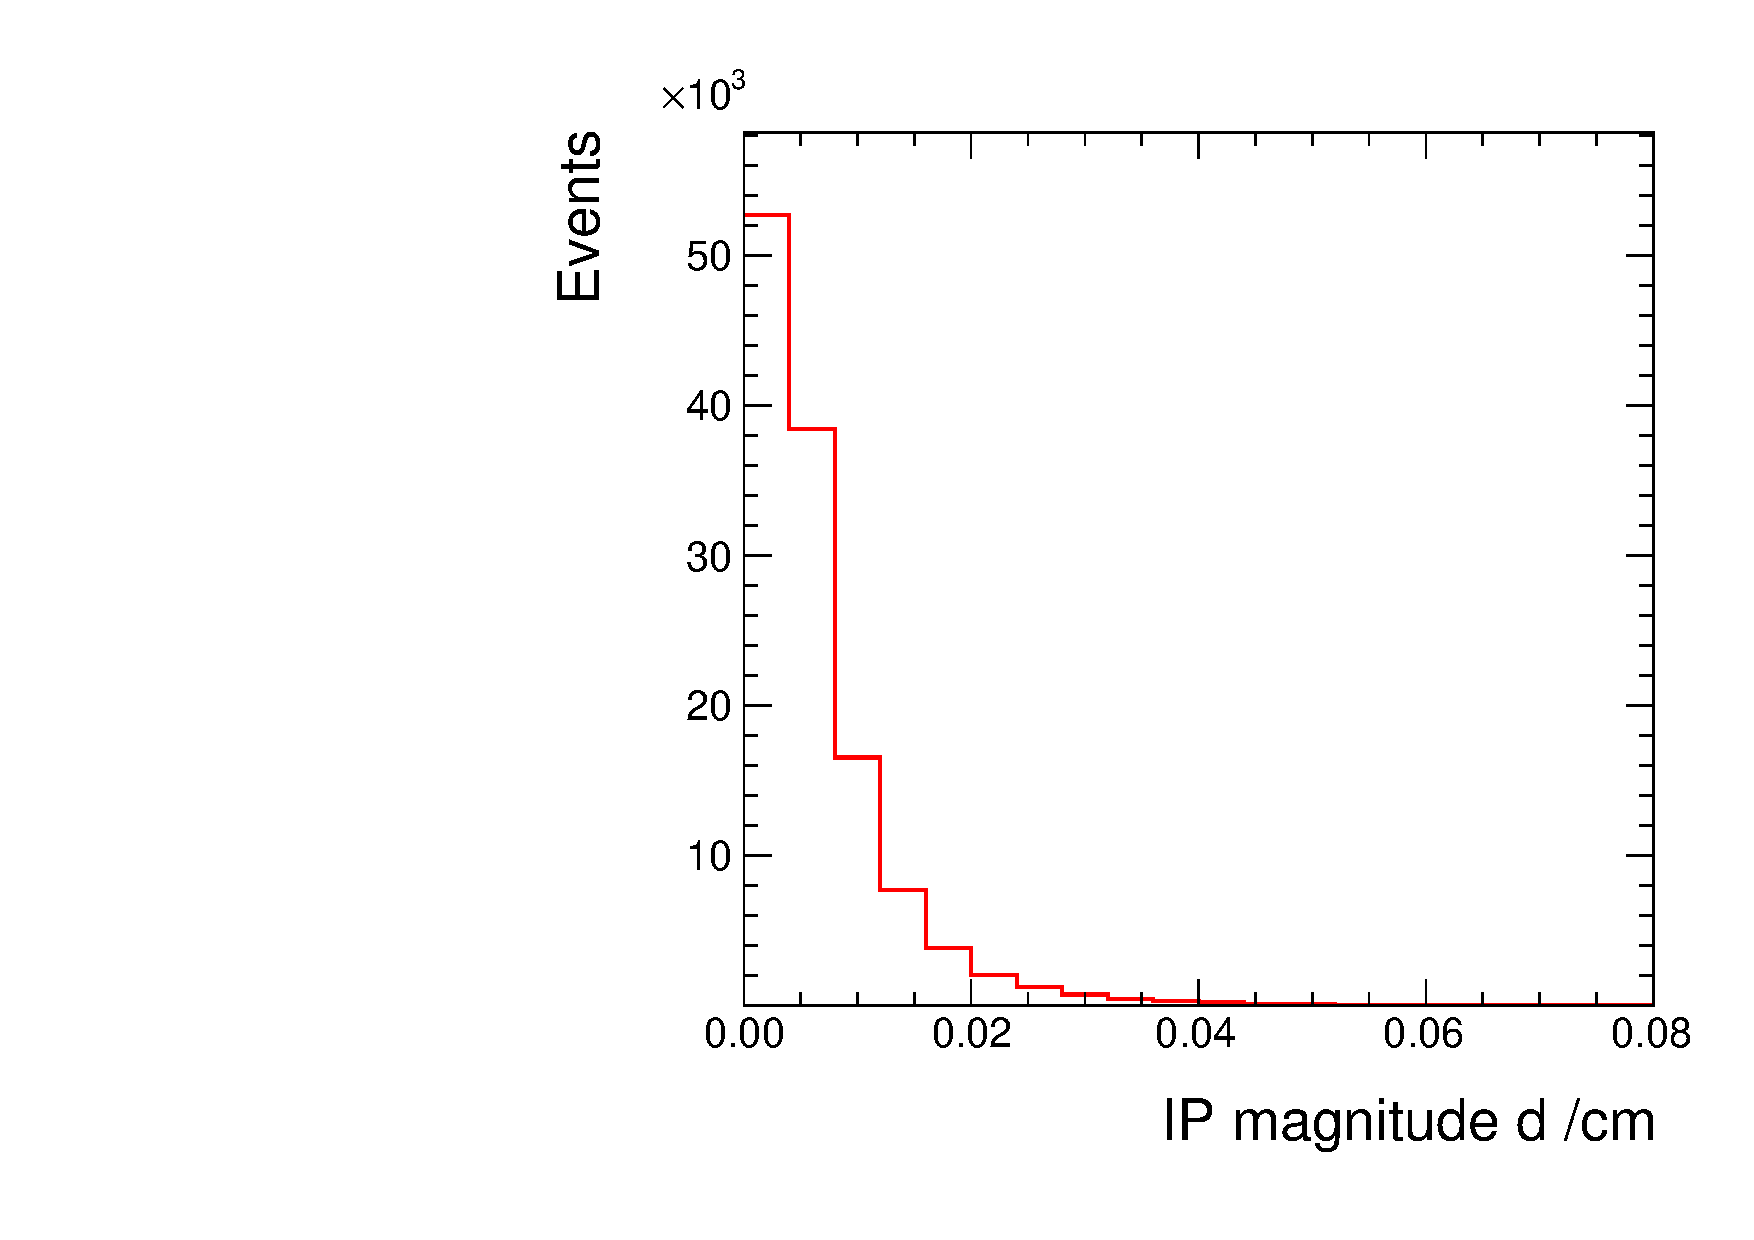
\includegraphics[width=0.4\linewidth]{Figures/IP_mag.pdf}}
	\subfigure{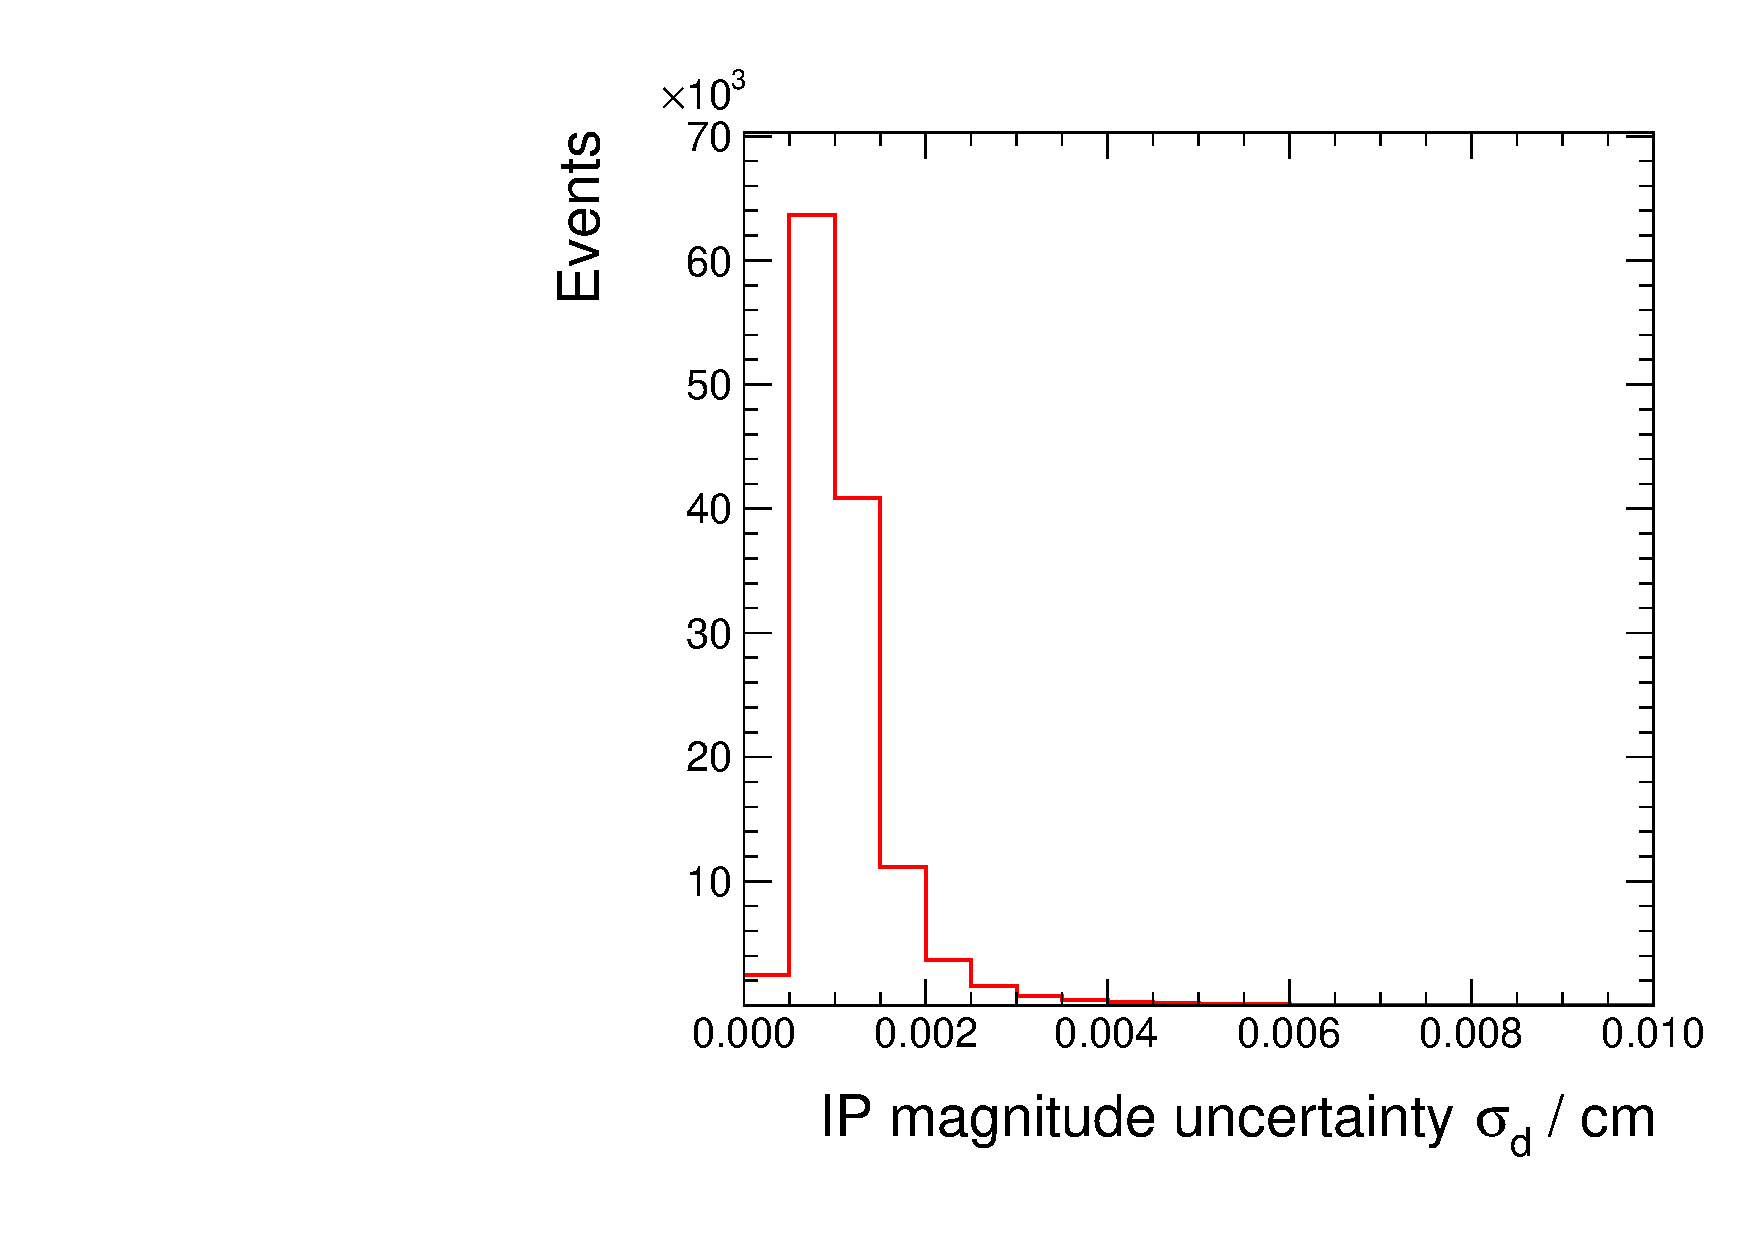
\includegraphics[width=0.4\linewidth]{Figures/IP_mag_err.pdf}}
	\caption{The distribution of IP vector magnitudes $d$ and its uncertainty $\sigma_{d}$ originating from the primary vertex in the $\mu\rho$ decay mode}
	\label{fig:lambda_dist}
\end{figure}
\begin{figure}[h]
	\centering
	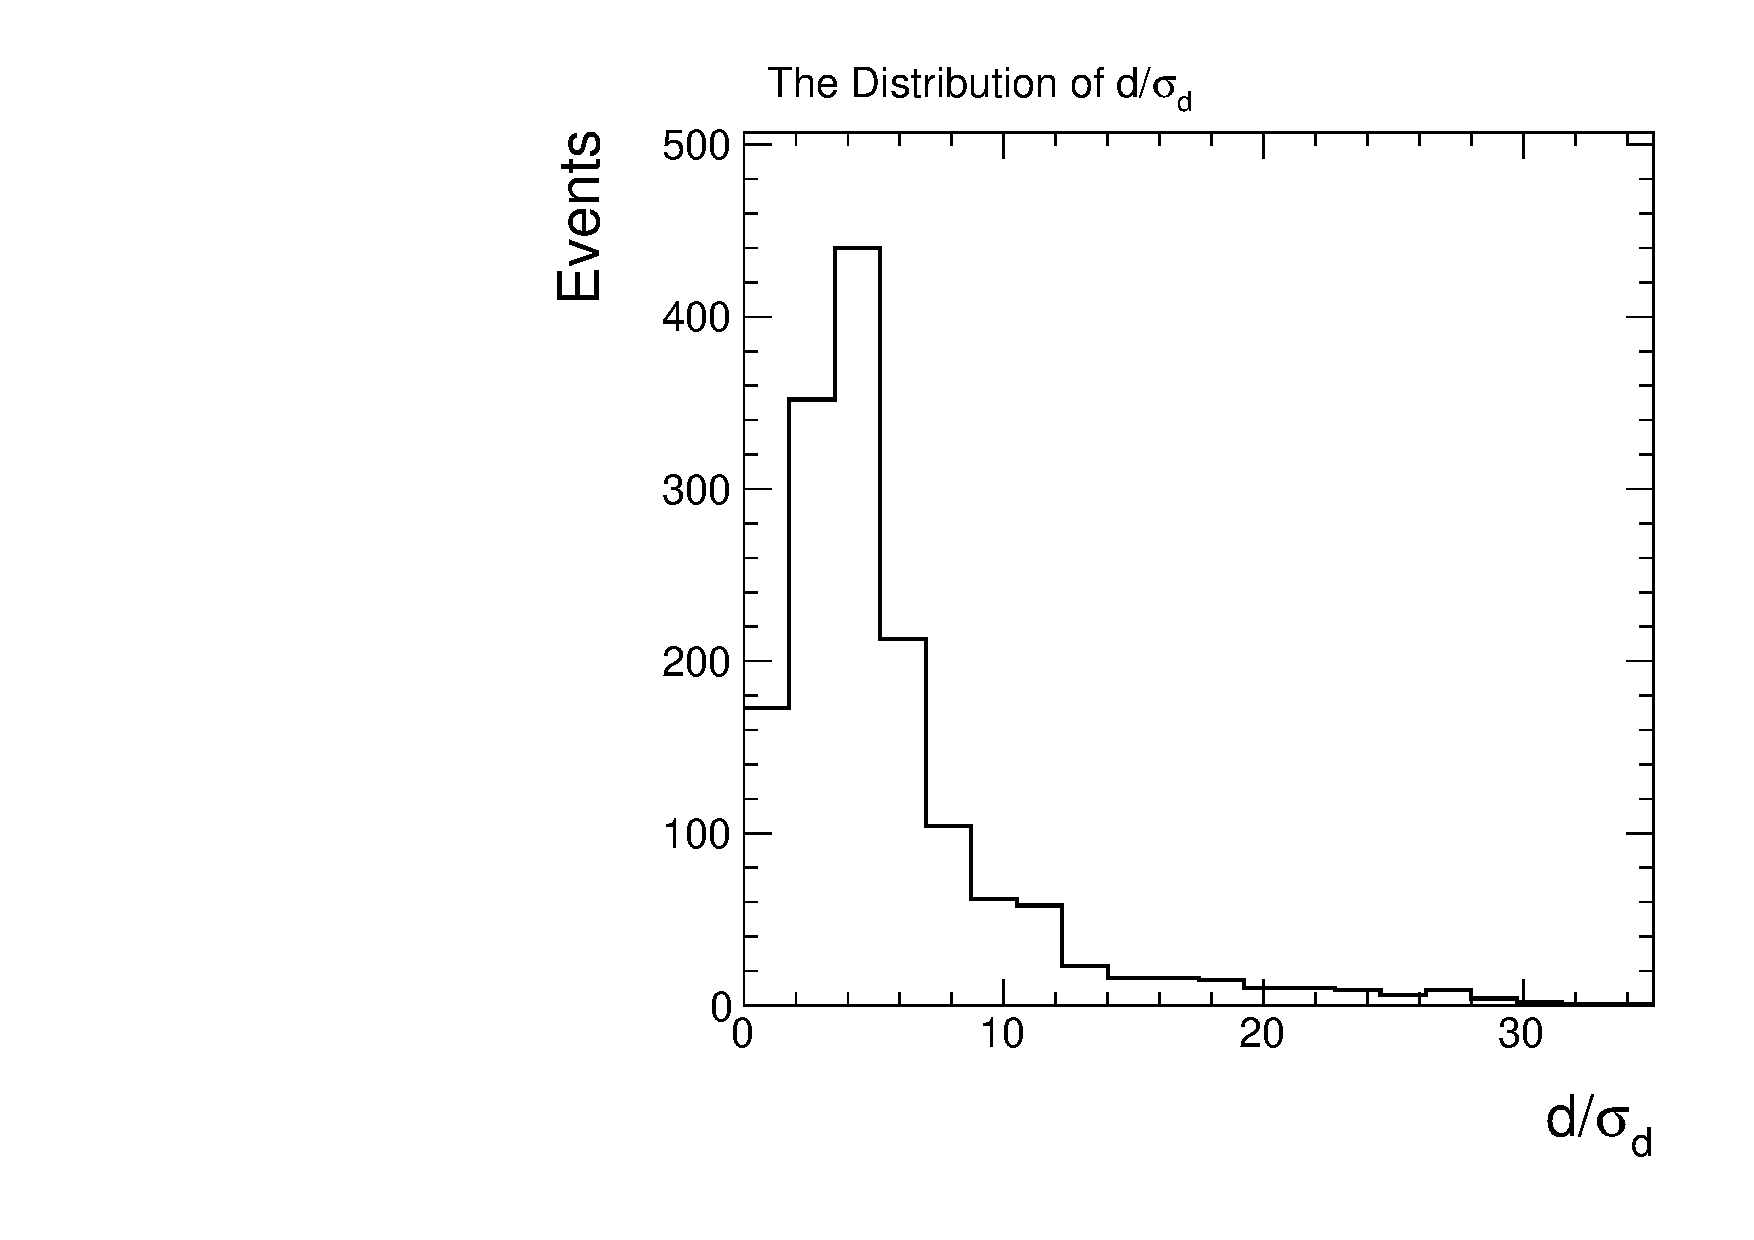
\includegraphics[width=0.6\linewidth]{Figures/IP_mag_IP_Over_err.pdf}
	\caption{The distribution of $\frac{d}{\sigma_d}$ in the $\mu \rho$ decay mode}
	\label{fig:IP_magOverLambda_dist}
\end{figure}
\begin{figure}[h]
	\centering
	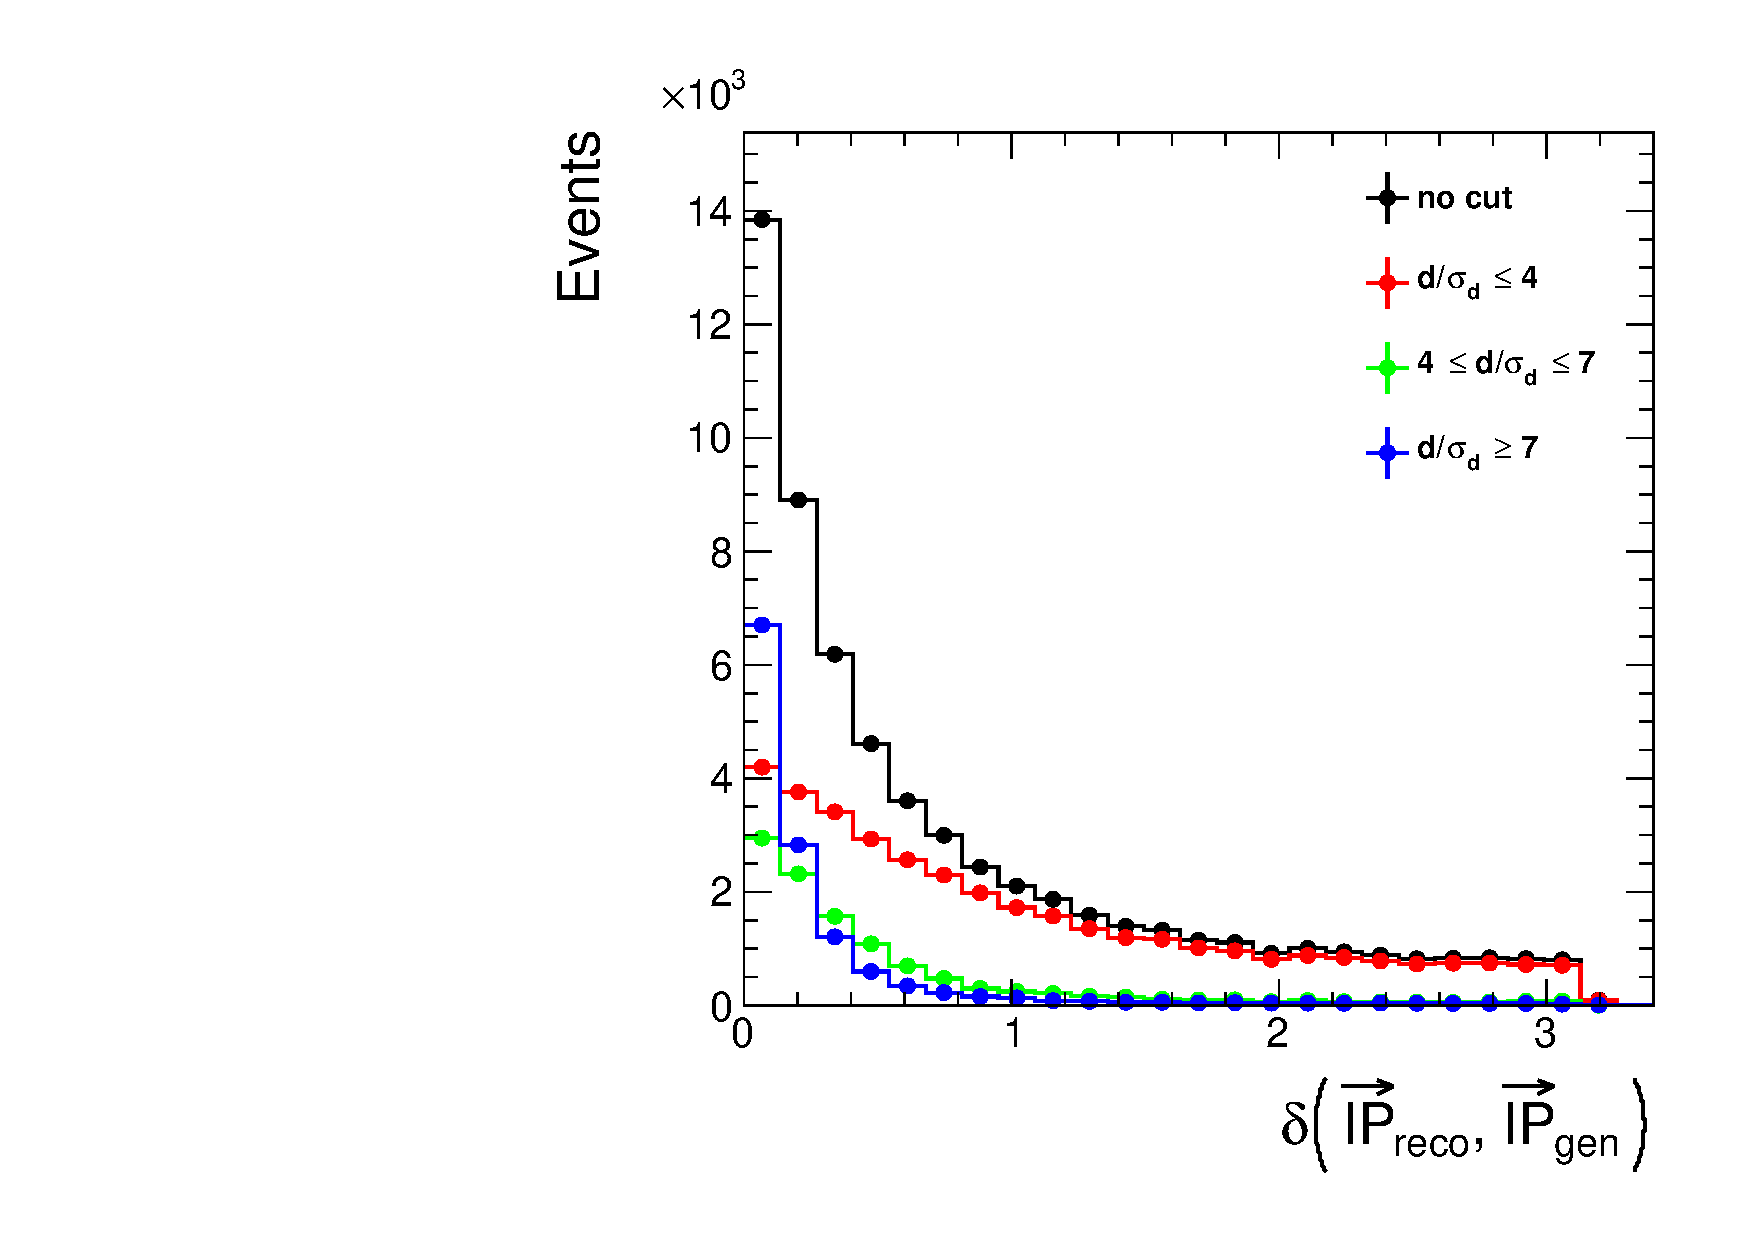
\includegraphics[width=0.7\linewidth]{Figures/deltaGenRecoIP1.pdf}
	\caption{The study of the 3D angle between the generated and reconstructed IP vectors in the $\mu\rho$ decay mode. One can observe the steady disappearance of events with small IP vectors with respect to the uncertainty ellipsoid.}
	\label{fig:lambdacuts_angles}
\end{figure}
\begin{figure}[h]
	\centering
	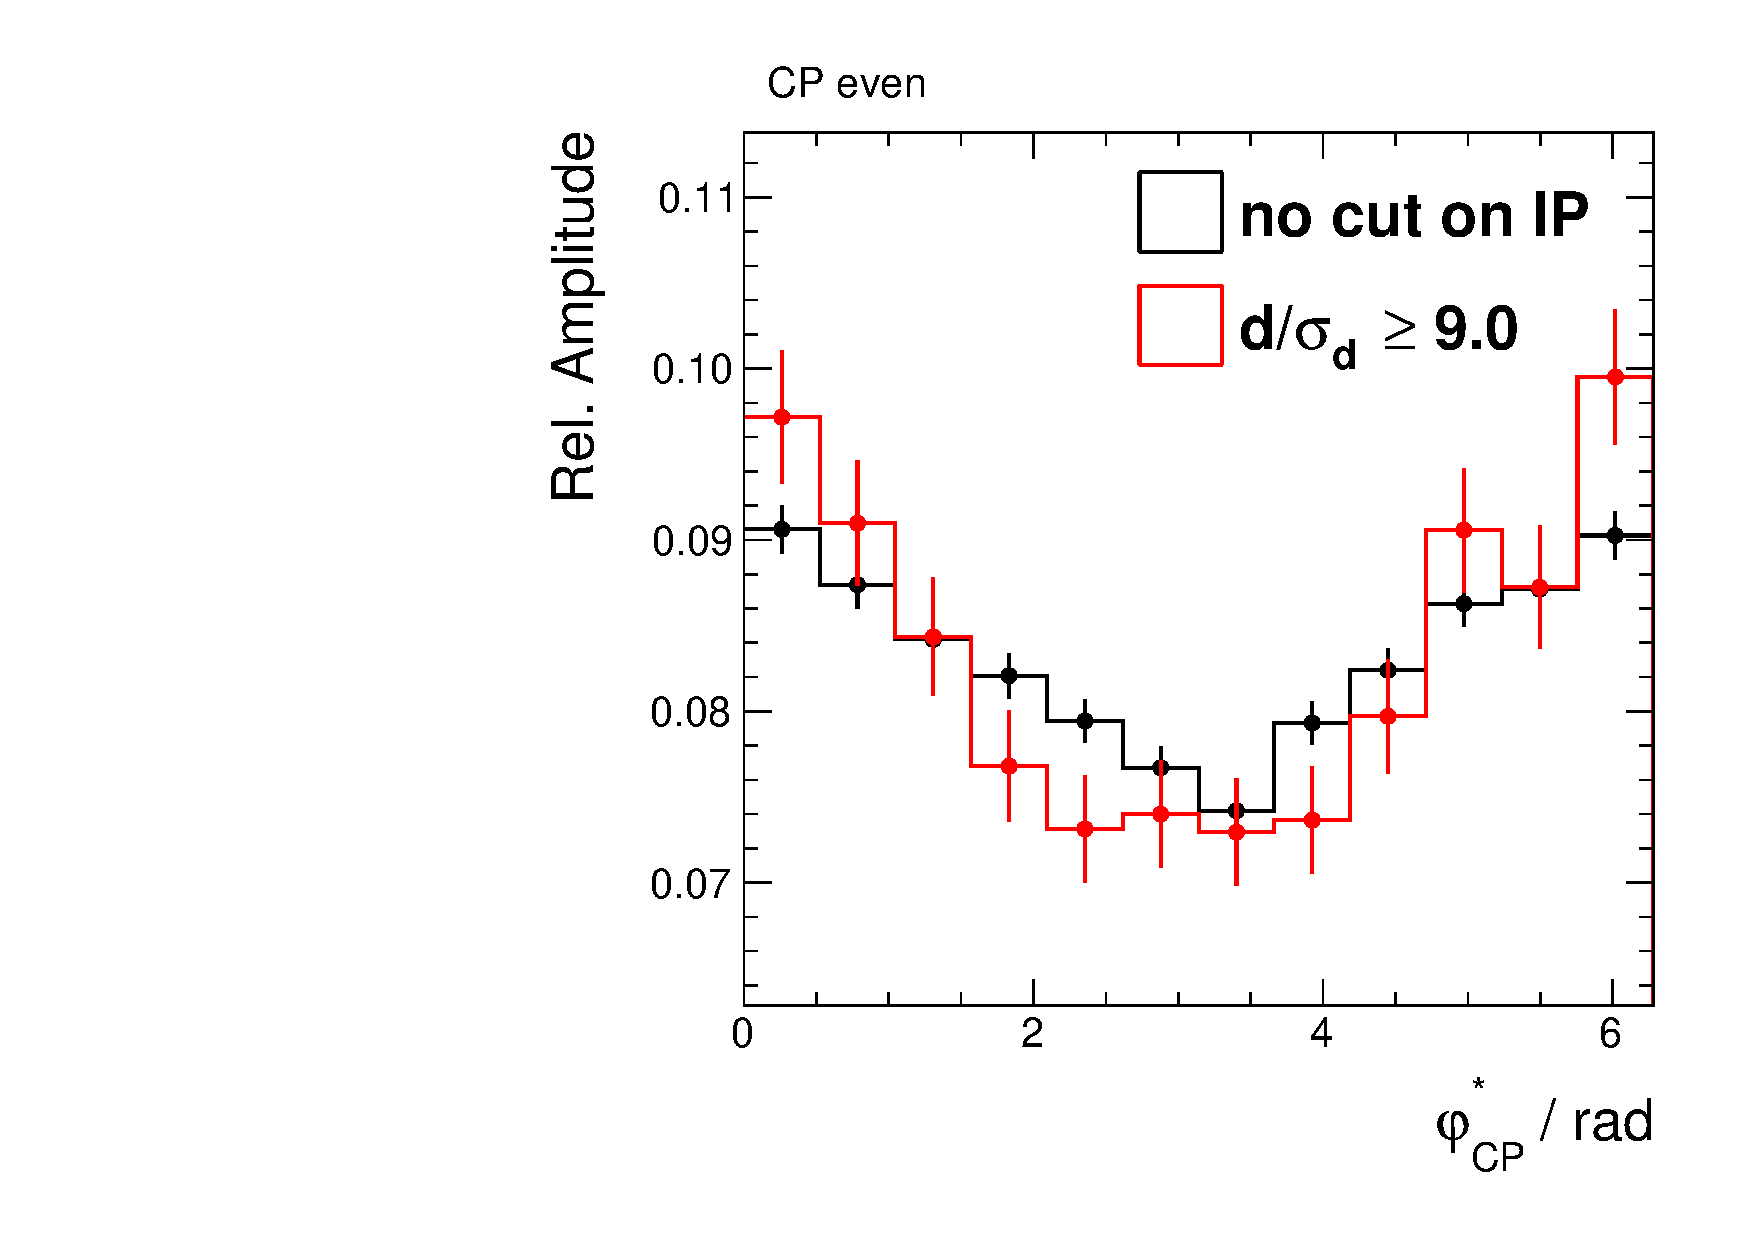
\includegraphics[width=0.7\linewidth]{Figures/recoPhiStarCPCombMerged_norefit_CPeven.pdf}
	\caption{The influence of $\alpha$-cuts on a CP-even scenario in the $\mu\rho$ decay mode. The influence of the selection of well-reconstructed decay planes can be immediately seen by the increase in the amplitude of the distribution in red.}
	\label{fig:lambdacuts_CP}
\end{figure}\\
To summarise, an efficient way of event selection has been found, which helps to reduce the influence of the primary vertex uncertainty concerning the direction of the IP vector. In order to complete the analysis, one should not neglect the uncertainty ellipsoid around the "other end" of the PV vector, which corresponds to a point on the track of the particle. Such an additional term however would only increase the total uncertainty with respect to $\sigma_{d}$ and therefore the influence of $\alpha$ on the distribution $\frac{d}{\sigma_d}$.
\chapter{The Impact Parameter Method} % Main chapter title

\label{Chapter5} % For referencing the chapter elsewhere, use \ref{Chapter1} 

In Chapter \ref{Chapter4} one has studied the influence of the primary vertex uncertainty on the dataset. In the following, a new way of finding the impact parameter vector is going to be proposed and compared to the tangential approach \parencite{Claudia_thesis} currently in use by the \verb|Artus| framework.

\section{Theoretical background}
First of all, one has to find the track of the particle and a suitable parametrisation thereof. Since we are considering charged particles moving with a velocity \textbf{v} in a homogeneous magnetic field $\boldsymbol{B} = B\boldsymbol{e}_z$, one expects to find a helical trajectory. Evidently, cylindrical coordinates are the most elementary way to parametrize it, keeping the problem as simple as possible. In the following, a quick derivation of the trajectory is going to be discussed, since the parameters appearing in the equations of motion have to be uniquely identified with those used by the track fitting algorithm.\\
In order to find the track, consider a classical particle of charge $q$ as described above. On such a particle, the relativistic Lagrangian $\mathcal{L}$ (up to a gauge transformation) takes in cgs-Gaussian units the form \parencite{Jackson}
\begin{equation}
	\mathcal{L} = -mc^2\cdot\sqrt{1-\left(\frac{\dot{\boldsymbol{x}}}{c}\right)^2}+\frac{q}{c}( \boldsymbol{v}\cdot\mathbf{A})
\end{equation}
with the vector potential $\boldsymbol{A}$ satisfying $\boldsymbol{B} = \nabla \times \mathbf{A}$. In case of a homogeneous magnetic field, $\boldsymbol{A}$ can be written (up to a gauge transformation) as
\begin{equation}
	\mathbf{A} = \frac{B}{2}\left(\begin{tabular}{c}
	$-y $\\ 
	$x$\\ 
	$0$
	\end{tabular} \right)
\end{equation}
leading to the Lagrangian
\begin{equation}
	\mathcal{L} = -mc^2\cdot\sqrt{1-\left(\frac{\dot{\boldsymbol{x}}}{c}\right)^2}+\frac{qB}{2c}( x\dot{y} - y\dot{x}),
\end{equation}
which can be rewritten in SI units as
\begin{equation}
	\mathcal{L} = -mc^2\cdot\sqrt{1-\left(\frac{\dot{\boldsymbol{x}}}{c}\right)^2}+\frac{qB}{2}( x\dot{y} - y\dot{x}).
\end{equation}\\
Using the variational principle, the action $S =\int\mathcal{L}dt$ is stationary if and only if $\mathcal{L}$ fulfils the Euler-Lagrange equations yielding the following set of equations of motion:
\begin{center}
	$\left\lbrace
	\begin{aligned}
		-qB\dot{x}&=m\gamma\ddot{y}\\
		qB\dot{y}&=m\gamma\ddot{x}\\
		0&=mg\ddot{z}
	\end{aligned}
	\right.$
\end{center}
where $\gamma$ denotes the Lorentz-gamma. The ansatz
\begin{equation}
	\boldsymbol{x}(t) = \boldsymbol{O'} +  \left(\begin{tabular}{c}
	$R\cos(\omega t + \varphi_1) $\\ 
	$-R\sin(\omega t + \varphi_1) $\\ 
	$v_z t $
	\label{eq:ansatz}
	\end{tabular} \right)
\end{equation}
(where \textbf{O'} is a constant vector) is indeed a solution to the problem. Putting this ansatz in the equations of motion provides the correspondence between the magnitude of the elements of the 4-momentum $p^\mu$, the particle charge $q$ and the geometrical parameter $\omega$, the angular frequency given by $\omega = \frac{qB}{m\gamma}$. Considering the magnitude of the relativistic 3-momentum of a such particle yields the expression between the radius $R$ and $p$, given by $R=\frac{p_T}{qB}=\frac{p\sin\theta}{qB}$, where $\theta$ denotes the polar angle.\\
Having expressed $R$ and $\omega$ through the measurable physical variables $p, B$ and $m\gamma$ (which can be derived from the total energy of the particle), now one can move to the helix reconstruction algorithm, which executes a fit with respect to the following parameters:
\begin{itemize}
	\item $\frac{q}{p}$: the signed inverse of the momentum at a reference point \textbf{R} $=(R_x, R_y, R_z)$ defined as the closest point on the helix to the center of the detector
	\item $\lambda = \frac{\pi}{2} - \theta$ ; $\lambda \in [0, \pi)$: the polar angle of the 3-momentum in \textbf{R} to XY-plane
	\item $\varphi \in [-\pi,\pi)$: the azimuth angle of the 3-momentum vector in the point \textbf{R} in the XY-plane with respect to the x-axis
	\item $d_{xy} = -R_x \sin\varphi + R_y \cos\varphi$: the signed distance between the tangent of the helix in \textbf{R} and the origin in the XY-plane
	\item $d_{sz} = R_z\cos\lambda - (R_x\cos\varphi+R_y\sin\varphi)\sin\lambda$: defined in the SZ-plane, where S denotes to the distance travelled by the particle in the XY-plane
\end{itemize}
A visualisation of these parameters can be found in Fig. \ref{fig:geometry}, where $v$ corresponds to the primary vertex of $\tau$-production (which is with a very good approximation the same as the production vertex of the Higgs-boson) and $\boldsymbol{O'}$ is the projected rotation axis of the helix. By using the above parametrisation, one has also to take into account that $\varphi_1$ is positive in the negative $\varphi$ region; this has the advantage that positively charged particles move to the direction of increasing $\varphi_1$. Obviously, one could have taken a trigonometric argument of the form $(\omega t-\varphi_1)$ with an oppositely signed angle $\varphi_1$ -- this is just matter of convention.
\begin{figure}[h]
	\centering
	\begin{tikzpicture}
	\centering
	
	\def\centerarc[#1](#2)(#3:#4:#5)% Syntax: [draw options] (center) (initial angle:final angle:radius)
	{ \draw[#1] ($(#2)+({#5*cos(#3)},{#5*sin(#3)})$) arc (#3:#4:#5); }
	
	\draw[thick,->, name path = x_axis_line] (-1,0) -- (10,0) node[anchor=north west] (x_axis) {x};
	\draw[thick,->] (0,-1) -- (0,4) node[anchor=south east] {y};
	\fill (0,0) circle (2pt) node[anchor=north east]{O};
	%\draw [name path = c] (8,6) circle (4);
	\centerarc[name path = c](8,6)(170:260:6);
	\path [name path = Op,draw] (0,0) -- (8,6) coordinate (Op_point);
	\node[anchor=north] at (2,1.5) {$d_{xy}$};
	\draw[dashed, name path = horizontal_Op] (7.5,6)--(10,6)  coordinate (horizontal_Op_line);
	\fill (8,6) circle (2pt) node[anchor=south]{O'};
	\fill [name intersections={of=Op and c}]
	(intersection-1) circle (2pt) node[anchor=east] {R} coordinate (R);
	\draw[dashed, name path = tangent_line] (intersection-1) --++(4,-5.33) coordinate (tangent);
	\draw[line width=0.6mm,->] (intersection-1) --++(0.5,-0.66) node [anchor=east] {$\boldsymbol{p}_T$};
	\draw[dashed] (intersection-1) --++(-3,4); %(3,-4)
	\fill [name intersections={of=tangent_line and x_axis_line}]
	(intersection-1) circle (0pt) coordinate[anchor=north east] (inter);
	\draw[dashed] (intersection-1) --++(-3,4);
	\pic [draw, <-, "$\varphi$", angle eccentricity=0.6,angle radius=11mm] {angle = tangent--inter--x_axis};
	%PV:
	\draw[->] (0,0) -- (2,3);
	\node[anchor=south] at (0.8,1.5) {$\boldsymbol{v}$};
	\pic [draw, <-, "$\varphi_1$", angle eccentricity=0.6,angle radius=5mm] {angle = R--Op_point--horizontal_Op_line};
	\end{tikzpicture}
	\caption{a visualisation of fit parameters, for a negatively charged particle in the XY-plane; here $\boldsymbol{v}$ is the PV-vector and $\varphi_1>0$ and $\varphi<0$}
	\label{fig:geometry}
\end{figure}\\
As introduced in section \ref{sec:IP_method} in the gluon-gluon fusion process, the impact parameter is a $CP$-sensitive variable enabling us to determine the angle $\varphi^*$. Nevertheless, a direct measure of this vector is not possible, hence it is necessary to calculate it, whereas multiple approaches can be considered. In this thesis, two of them are going to be discussed: the so-called tangential approximation \parencite{Claudia_thesis} and the helical approximation.\\

\section{The tangential approximation}
A typical particle produced in the CMS-experiment is highly relativistic, which leads to extremely great curvatures and radii $R$ compared to the scale of the IP. Therefore, one could approximate in the close neighbourhood in the region of the secondary vertex (the $\tau$-decay vertex) the helical trajectory with a straight line. Assuming the primary vertex is close to the centre of the detector (the origin) one could utilise the above introduced reference point \textbf{R} to extrapolate the trajectory linearly along $\lambda$ and $\varphi$.\\
\begin{figure}[h]
	\centering
	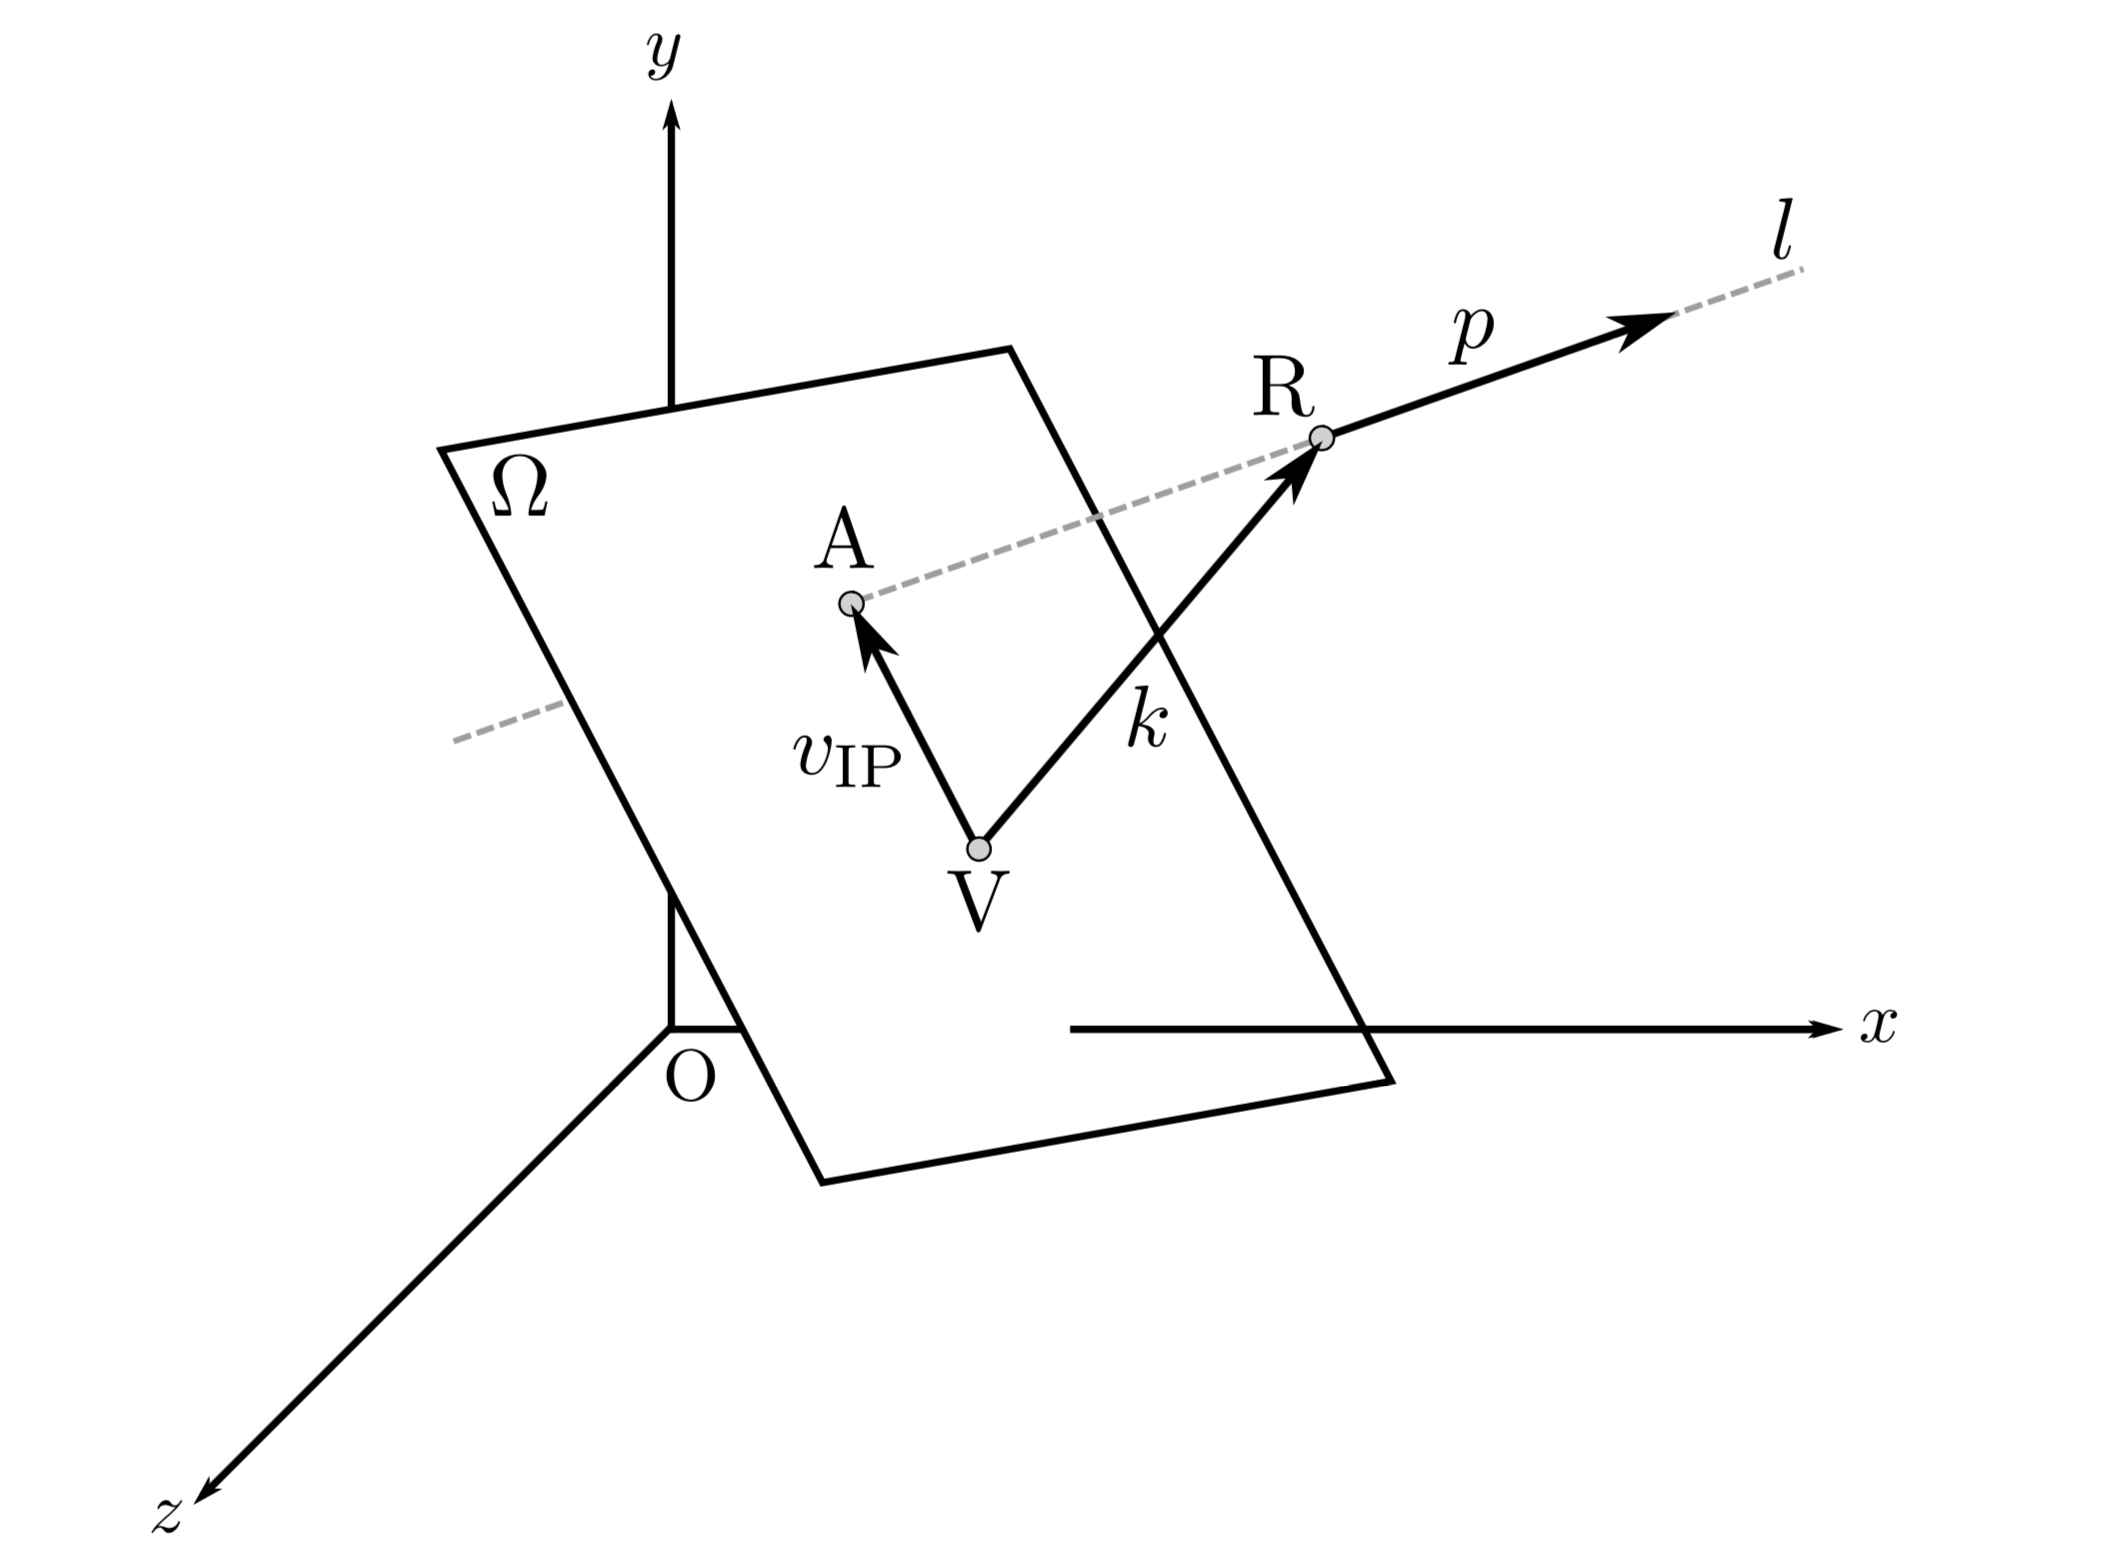
\includegraphics[width=0.5\linewidth]{Figures/IP_tangential}
	\caption{The geometry of finding the IP-vector (here denoted as $v_{IP}$). Source: \parencite{Claudia_thesis}}
	\label{fig:iptangential}
\end{figure}\\
To determine the IP with this method, consider Fig. \ref{fig:iptangential}, where V is the primary vertex. From the definition of the impact parameter follows that the distance between the straight line defined by the 3-momentum vector $\boldsymbol{p}$ of the lepton $l$ at \textbf{R} and the primary vertex point V should be minimised. In other terms, the IP-Vector $\boldsymbol{v}_{IP}$ should stay orthogonal to the (normalised) momentum vector $\boldsymbol{\hat{p}}$ meaning
\begin{equation}
	\boldsymbol{v}_{IP} \cdot \boldsymbol{\hat{p}} = 0.
\end{equation}
Nevertheless, the vector $\overrightarrow{VA}$ can be expressed as
\begin{equation}
	\overrightarrow{VA} = \boldsymbol{v}_{IP} = \boldsymbol{k}+\alpha \cdot \boldsymbol{\hat{p}},
\end{equation}
with an $\alpha \in \mathbb{R}$. Combining the two conditions yields
\begin{equation}
	\alpha = -\boldsymbol{k}\cdot\boldsymbol{\hat{p}}
\end{equation}
which then can be used to determine the $\boldsymbol{v}_{IP}$:
\begin{equation}
	\boldsymbol{v}_{IP} = \boldsymbol{k}-(\boldsymbol{k}\cdot\boldsymbol{\hat{p}})\boldsymbol{\hat{p}}
\end{equation}
There are however multiple problems with such an approach. First, it uses a physically meaningless point \textbf{R} to obtain a crucial physical parameter, $\boldsymbol{v}_{IP}$. Second, it does not take the curvature of the particle trajectory into account, leading to errors. Third, and most importantly, the basic assumption (about the position of the primary vertex) on which this algorithm lies upon, does not necessarily hold, see \ref{fig:PVs}. In this figure, one can immediately observe that the position of the primary vertices is of the same order of magnitude as the length of the impact parameter vectors (see \ref{fig:lambda_dist}). Therefore, a further study of IP-reconstruction needs to be considered.\\
\begin{figure}[h]
	\centering
	\subfigure{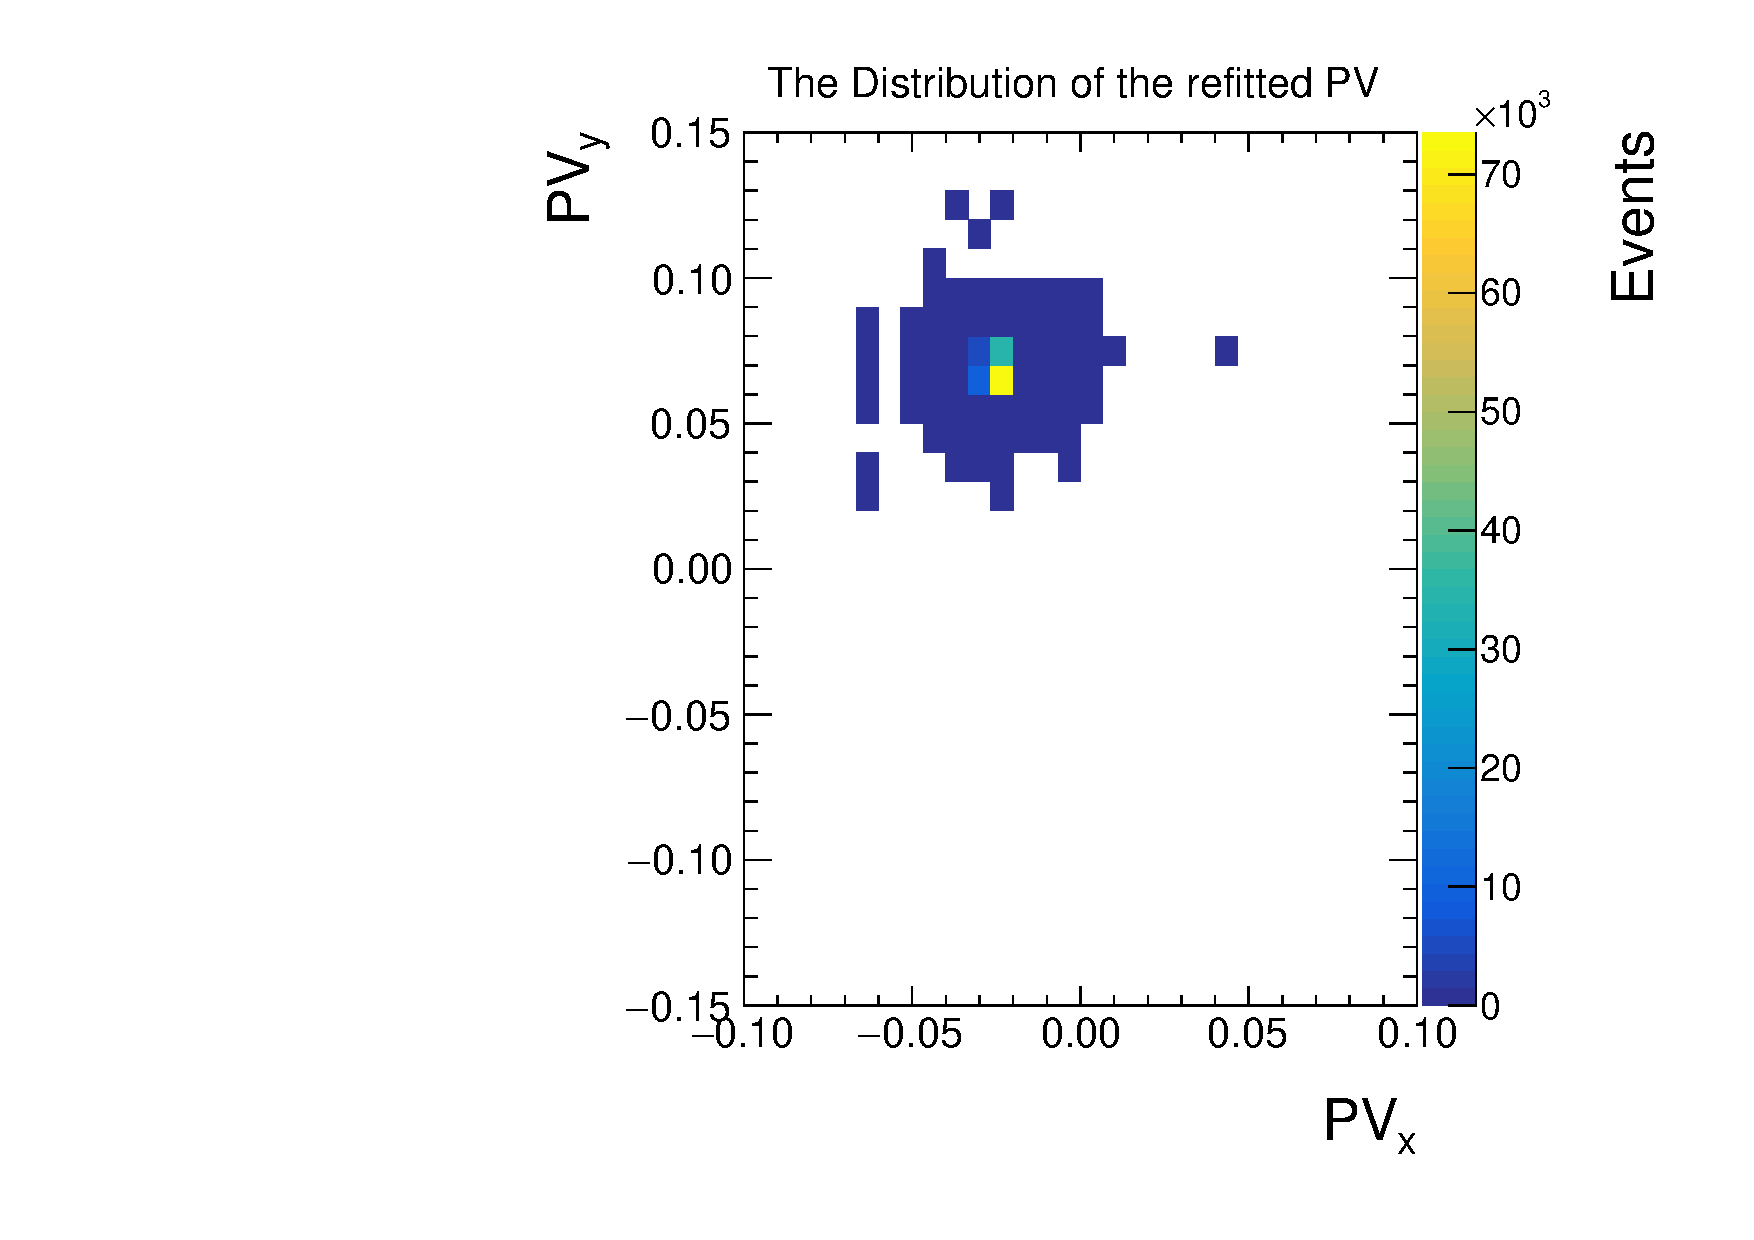
\includegraphics[width=0.4\linewidth]{Figures/PVs}}
	\subfigure{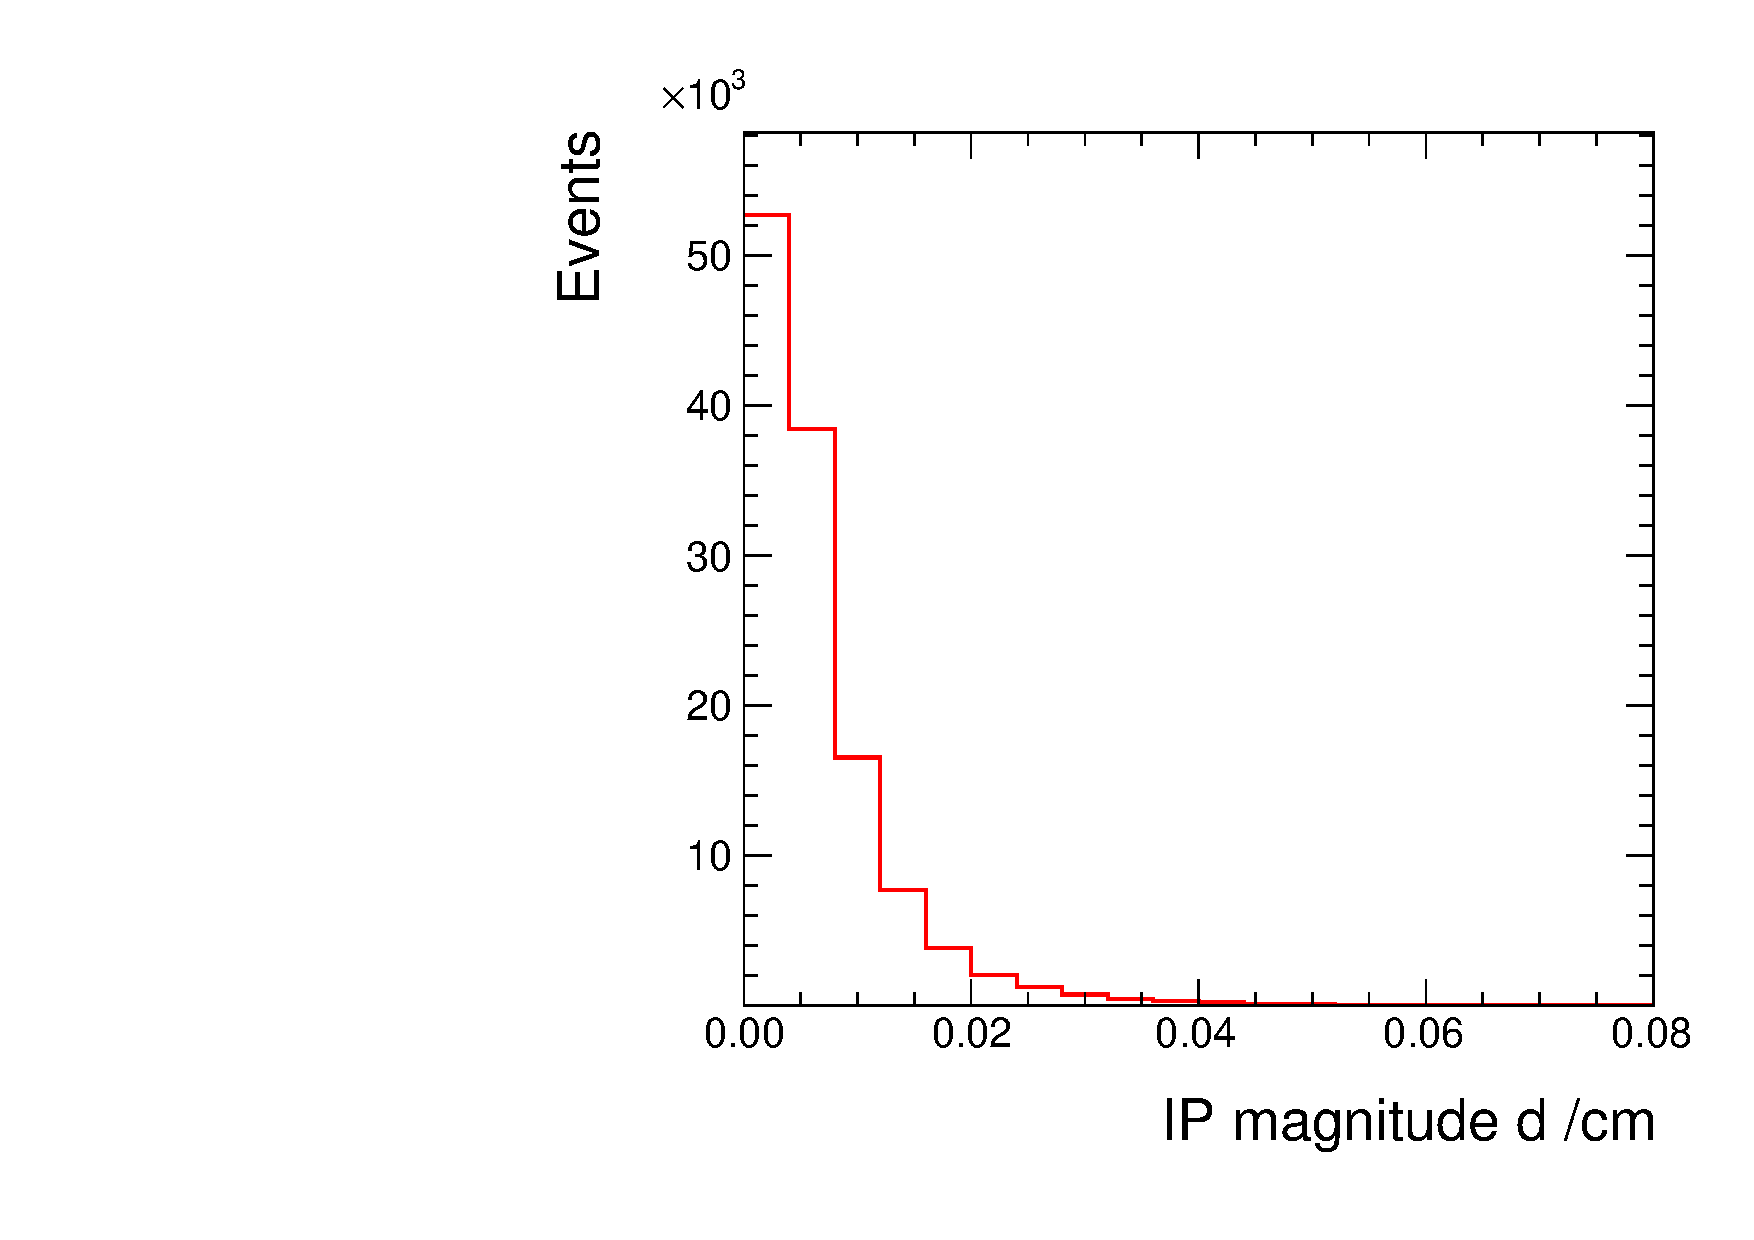
\includegraphics[width=0.4\linewidth]{Figures/IP_mag.pdf}}
	\caption{Left: The positions of the refitted primary vertices of the Higgs decays\\Right: The Distribution of IP-Magnitudes in all decay channels}
	\label{fig:PVs}
\end{figure}
\newpage
\section{The helical approximation}
Given the fact that both the $\tau$ particles and the secondary vertices cannot be precisely reconstructed, one needs to find a point which lies as closely to the latter, as possible. Another assumption is the consideration of the point of closest approach (PCA) of the particle on its trajectory as the base of IP-reconstruction. Having defined the IP-vector as the vector pointing from the primary vertex V to the PCA and considering the helix parametrised as in Eq. \ref{eq:ansatz}, it is simple to obtain the newly defined impact parameter, by minimising
\begin{equation}
	\delta(t) = |\boldsymbol{x}(t)-\boldsymbol{v}|^2,
\end{equation}
in $t$, where \textbf{v} denotes the vector pointing from the origin to V. Since $\delta(t)$ is a smooth function with existing higher-order derivatives, the problem can be  calculated numerically.
\subsection{Implementation}
Nevertheless, comparing the fit parameters with Eq. \ref{eq:ansatz}, one first needs to find a bijection between the two parametrisations. However, since both $R$ and $\omega$ are known from the particle's properties, it remains only to determine \textbf{O'}, $\varphi_1 \in [-\pi,\pi)$ and $v_z$.
\paragraph{Finding $\varphi_1$}\mbox{}\\
While determining $\varphi_1$, it has to be taken into consideration that only the $\varphi$-component of the tangent in \textbf{R} is known, from which $\varphi_1$ cannot be easily obtained just by adding or subtracting $\pi/2$. An example of this problem is visualised in Fig. \ref{fig:geometry2}. In this two independent cases portrayed here, one can obtain $\tilde{\varphi_1}$ from $\tilde{\varphi}$ via $\tilde{\varphi_1}=-\tilde{\varphi}+\frac{\pi}{2}$ (keeping the sign convention of Eq. \ref{eq:ansatz} in mind). However, in case of $\hat{\phi}$ and $\hat{\phi_1}$ this relation becomes $\hat{\phi_1} = -\hat{\phi}$. For this reason, one needs to consider different cases separately.
\begin{figure}[h]
	\centering
	\begin{tikzpicture}
	\centering
	
	\def\centerarc[#1](#2)(#3:#4:#5)% Syntax: [draw options] (center) (initial angle:final angle:radius)
	{ \draw[#1] ($(#2)+({#5*cos(#3)},{#5*sin(#3)})$) arc (#3:#4:#5); }
	
	\draw[thick,->, name path = x_axis_line] (-8,0) -- (5,0) node[anchor=north west] (x_axis) {x};
	\draw[thick,->] (0,-1) -- (0,4) node[anchor=south east] {y};
	\fill (0,0) circle (2pt) node[anchor=north east]{O};


	\centerarc[name path = c](-8,6)(300:350:6);
	\path [name path = Op,draw] (0,0) -- (-8,6) coordinate (Op_point);
	\draw[dashed, name path = horizontal_Op] (-8.5,6)--(-7,6)  coordinate (horizontal_Op_line);
	\fill (-8,6) circle (2pt) node[anchor=south]{$\hat{O'}$};
	\fill [name intersections={of=Op and c}]
	(intersection-1) circle (2pt) node[anchor=west] {$\hat{R}$} coordinate (R);
	\draw[dashed, name path = tangent_line] (intersection-1) --++(-3,-4);
	\draw[dashed] (intersection-1) --++(3,4) coordinate (tangent);
	\draw[line width=0.6mm,->] (intersection-1) --++(0.5,0.66) node [anchor=east] {$\boldsymbol{\hat{p}}_T$};
	\fill [name intersections={of=tangent_line and x_axis_line}]
	(intersection-1) circle (0pt) coordinate[anchor=north east] (inter);
	\pic [draw, ->, "$\hat{\varphi}$", angle eccentricity=0.6,angle radius=11mm] {angle =x_axis--inter--tangent};
	\pic [draw, <-, "$\hat{\varphi_1}$", angle eccentricity=0.6,angle radius=12mm] {angle = R--Op_point--horizontal_Op_line};
	

	%\draw [name path = c] (8,6) circle (4);
	\centerarc[name path = c](4,3)(170:260:3);
	\path [name path = Op,draw] (0,0) -- (4,3) coordinate (Op_point);
	\draw[dashed, name path = horizontal_Op] (3.5,3)--(5,3)  coordinate (horizontal_Op_line);
	\fill (4,3) circle (2pt) node[anchor=south]{$\tilde{O'}$};
	\fill [name intersections={of=Op and c}]
	(intersection-1) circle (2pt) node[anchor=east] {$\tilde{R}$} coordinate (R);
	\draw[dashed, name path = tangent_line] (intersection-1) --++(2,-2.66) coordinate (tangent);
	\draw[line width=0.6mm,->] (intersection-1) --++(0.5,-0.66) node [anchor=east] {$\boldsymbol{\tilde{p}}_T$};
	\draw[dashed] (intersection-1) --++(-3,4); %(3,-4)
	\fill [name intersections={of=tangent_line and x_axis_line}]
	(intersection-1) circle (0pt) coordinate[anchor=north east] (inter);
	\draw[dashed] (intersection-1) --++(-3,4);
	\pic [draw, <-, "$\tilde{\varphi}$", angle eccentricity=0.6,angle radius=11mm] {angle = tangent--inter--x_axis};
	\pic [draw, <-, "$\tilde{\varphi_1}$", angle eccentricity=0.6,angle radius=5mm] {angle = R--Op_point--horizontal_Op_line};
	\end{tikzpicture}
	\caption{Visualisation of the two cases for two different negatively charged particles}
	\label{fig:geometry2}
\end{figure}\\
First consider a negatively charged particle following a rotatory trajectory in a positive direction $\varphi$ in the XY-plane. For such a particle, one could rotate the normalised tangent vector at \textbf{R} with $\pi/2$ in the negative rotatory direction and consider the newly constructed radial vector $\hat{\boldsymbol{r}}$. However, the angle between this vector and the x-axis corresponds to the angle $\varphi_1$ we are looking for; in case of a positively charged particle, one could use the "mirrored version" of this method by rotating the tangent vector in the positive direction. Therefore, there are only these two cases to be considered, based on the charge of the particle.
\begin{figure}[h]
	\centering
	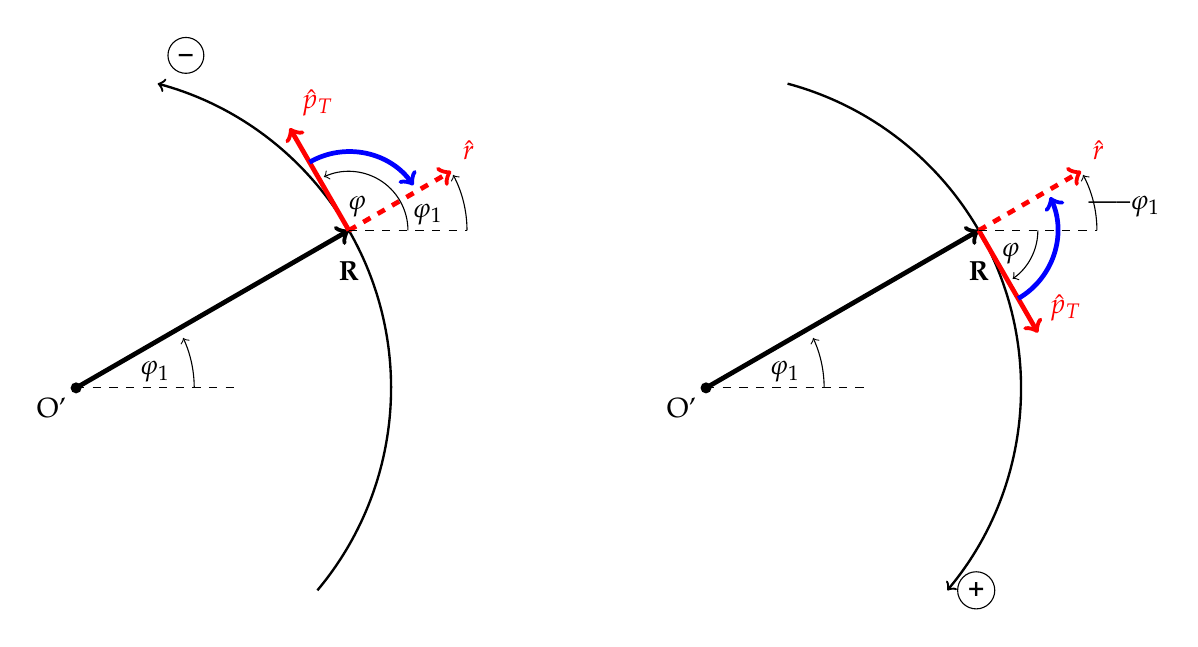
\begin{tikzpicture}
		\centering
		
		\def\centerarc[#1](#2)(#3:#4:#5)% Syntax: [draw options] (center) (initial angle:final angle:radius)
		{ \draw[#1] ($(#2)+({#5*cos(#3)},{#5*sin(#3)})$) arc (#3:#4:#5); }
		
		\fill (-7,0) circle (2pt) node[anchor=north east]{O'};
		\draw[dashed] (-7,0)--(-5,0);
		\centerarc[->](-7,0)(0:25:1.5);
		\node at (-6,0.2) {$\varphi_1$};
		
		\centerarc[line width=0.3mm,->](-7,0)(-40:75:4);
		\node[anchor = south west] at ($(-7,0)+({4*cos(75)},{4*sin(75)})$) {\encircle{\textbf{--}}};
		\draw[line width=0.6mm,->] (-7,0)--++($({4*cos(30)},{4*sin(30)})$) node[below = 7pt] {\textbf{R}};
		\draw[line width=0.6mm,->,red] ($({-7+4*cos(30)},{4*sin(30)})$)--++($({-1.5*sin(30)},{1.5*cos(30)})$) node[anchor = south west] {$\hat{p}_T$};
		\draw[dashed, line width=0.6mm,->,red] ($({-7+4*cos(30)},{4*sin(30)})$)--++($({1.5*cos(30)},{1.5*sin(30)})$) node[anchor = south west] {$\hat{r}$};
		\draw[dashed] ($({-7+4*cos(30)},{4*sin(30)})$)--++(1.5,0);
		\centerarc[->]($({-7+4*cos(30)},{4*sin(30)})$)(0:115:0.75);
		\node at ($({-6.9+4*cos(30)},{0.3+4*sin(30)})$) {$\varphi$};
		\centerarc[->]($({-7+4*cos(30)},{0+4*sin(30)})$)(0:28:1.5);
		\node at ($({-6+4*cos(30)},{0.2+4*sin(30)})$) {$\varphi_1$};
		
		\centerarc[line width=0.6mm,->,blue]($({-7+4*cos(30)},{4*sin(30)})$)(120:35:1);
		
		
		\fill (1,0) circle (2pt) node[anchor=north east]{O'};
		\draw[dashed] (1,0)--(3,0);
		\centerarc[->](1,0)(0:25:1.5);
		\node at (2,0.2) {$\varphi_1$};
		
		\centerarc[line width=0.3mm,<-](1,0)(-40:75:4);
		\node[anchor = west] at ($(1,0)+({4*cos(-40)},{4*sin(-40)})$) {\encircle{\textbf{+}}};
		\draw[line width=0.6mm,->] (1,0)--++($({4*cos(30)},{4*sin(30)})$) node[below = 7pt] {\textbf{R}};
		\draw[line width=0.6mm,->,red] ($({1+4*cos(30)},{4*sin(30)})$)--++($({1.5*sin(30)},{-1.5*cos(30)})$) node[anchor = south west] {$\hat{p}_T$};
		\draw[dashed, line width=0.6mm,->,red] ($({1+4*cos(30)},{4*sin(30)})$)--++($({1.5*cos(30)},{1.5*sin(30)})$) node[anchor = south west] {$\hat{r}$};
		\draw[dashed] ($({1+4*cos(30)},{4*sin(30)})$)--++(1.5,0);
		\centerarc[->]($({1+4*cos(30)},{4*sin(30)})$)(0:-55:0.75);
		\node at ($({1.4+4*cos(30)},{-0.3+4*sin(30)})$) {$\varphi$};
		
		\centerarc[->]($({1+4*cos(30)},{4*sin(30)})$)(0:28:1.5);
		\node at ($({2.85+4*cos(30)},{0.3+4*sin(30)})$) {-----$\varphi_1$};
		
		\centerarc[line width=0.6mm,<-,blue]($({1+4*cos(30)},{4*sin(30)})$)(25:-60:1);
		\end{tikzpicture}
	%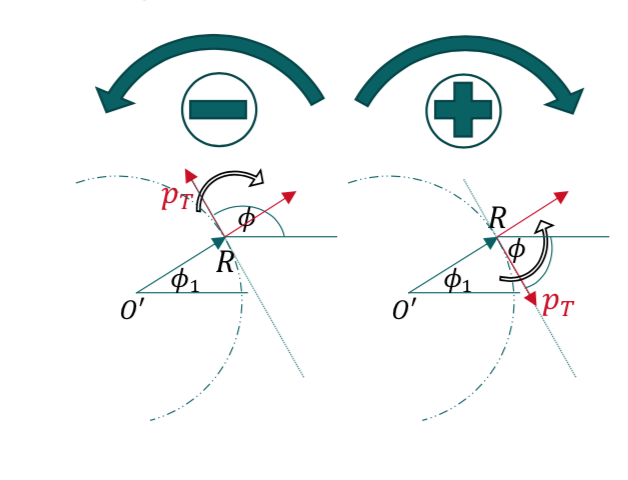
\includegraphics[width=0.7\linewidth]{Figures/rotations.png}
	\caption{Schematic representation of the determination of $\varphi_1$. Here the act of rotation is represented in blue.}
\end{figure}\\
In mathematical terms, let $\hat{\boldsymbol{p}}_T$ be the normalised 3-momentum vector projected to the XY-plane at $t=0$ for a positive particle. Then, the radial vector $\hat{\boldsymbol{r}}$ can be written with the rotation matrix $\textbf{R}_z (\phi)$ for an angle $\phi = \frac{\pi}{2}$ as
\begin{equation}
	\hat{\boldsymbol{r}} = \boldsymbol{R}_z\left(\phi = \frac{\pi}{2}\right)\,\hat{\boldsymbol{p}}_T = \begin{pmatrix}
	0 & -1 \\ 
	1 & 0 
	\end{pmatrix} \begin{pmatrix}
	\cos\varphi\\ 
	\sin\varphi
	\end{pmatrix} = \begin{pmatrix}
	-\sin\varphi\\ 
	\cos\varphi
	\end{pmatrix},
\end{equation}
so that the angle $|\varphi_1|$ between $\hat{\boldsymbol{r}}$ and the x-axis is given by the scalar product
\begin{center}
	\begin{tabular}{crl}
		&$\hat{\boldsymbol{r}} \cdot \boldsymbol{e}_x=$&$ -\sin\varphi= 1 \cdot 1\cdot\cos(|\varphi_1|)$\\
		\rule{0pt}{3ex}$\Rightarrow$&$\varphi_1 =$&$ \arccos(-\sin\varphi)\cdot(-\mathrm{sgn}(\hat{r}_y))$, \\ 
	\end{tabular} 
\end{center}
where the term $(-\mathrm{sgn}(\hat{r}_y))$ is due to the sign convention. Similarly, for a negatively charged particle, this yields
\begin{equation}
	\varphi_1 =\arccos(\sin\varphi)\cdot (-\mathrm{sgn}(\hat{r}_y)).
\end{equation}
The last two equations can be combined to obtain the relation between $\varphi_1$ and $\varphi$:
\begin{equation}
	\varphi_1 =\arccos(-\mathrm{sgn}(q)\sin\varphi)\cdot (-\mathrm{sgn}(\hat{r}_y))
\end{equation}
\paragraph{Finding \textbf{O'}}\mbox{}\\
In order to determine \textbf{O'}, one can use to the arbitrarily introduced parameter $t$ in the ansatz Eq. \ref{eq:ansatz}. Since the location of the particle is completely indifferent from the perspective of the IP-parameter problem, one can set the origin of time without any restrictions such that
\begin{equation}
	\boldsymbol{x}(0) = \boldsymbol{O'} +  \left(\begin{tabular}{c}
	$R\cos(\varphi_1) $\\ 
	$-R\sin(\varphi_1) $\\ 
	$0$\\
	\end{tabular} \right) \stackrel{!}{=} \boldsymbol{R}
\end{equation}
yielding
\begin{equation}
	\left\lbrace\begin{tabular}{ll}
	$O'_x =$&$R_x-R\cos(\varphi_1) $\\ 
	$O'_y =$&$R_y+R\sin(\varphi_1) $\\ 
	$O'_z =$&$R_z$\\
	\end{tabular} \right.
\end{equation}
which -- since $\varphi_1$ has already been found as a function of $\varphi$ and \textbf{R} is given by the fit algorithm -- is thereby uniquely defined.
\paragraph{Finding $v_z$}\mbox{}\\
Since the total momentum of the particle is given by $p = m\gamma v$, it follows
\begin{equation}
	v_z = \frac{p}{m\gamma}\cdot\cos\theta = \frac{p}{m\gamma}\cdot\cos\left(\frac{\pi}{2}-\lambda\right) =\frac{p}{m\gamma}\cdot -\sin(-\lambda) =  \frac{p}{m\gamma}\cdot\sin\lambda 
\end{equation}
\subsection{Results}
One way of judging the validity of a such theory is the comparison of the generator level dataset with the results obtained by this method on reconstruction level. This has been done in Fig. \ref{fig:deltaphinocut}, where the difference between the azimuthal angles $\Delta\phi$ between the IP on generator level and the differently reconstructed IP-vectors has been portrayed. In order to reduce uncertainties when dealing with such minimizer algorithms, this has been done with three different ones: the \verb|TMinimizer| of \verb|ROOT| utilises \verb|Minuit2|, a standard minimizer, the \verb|Brent|-algorithm, which is a combination of three different numerical minimizer algorithms (the bisection method, the secant method and the inverse quadratic interpolation). The third algorithm calculates an analytical solution by using a Taylor expansion of the helix for small $\omega t$-values, as discussed in Appendix \ref{AppendixA}, which delivers only approximative information about the overall distribution.
\begin{figure}[h]
	\centering
	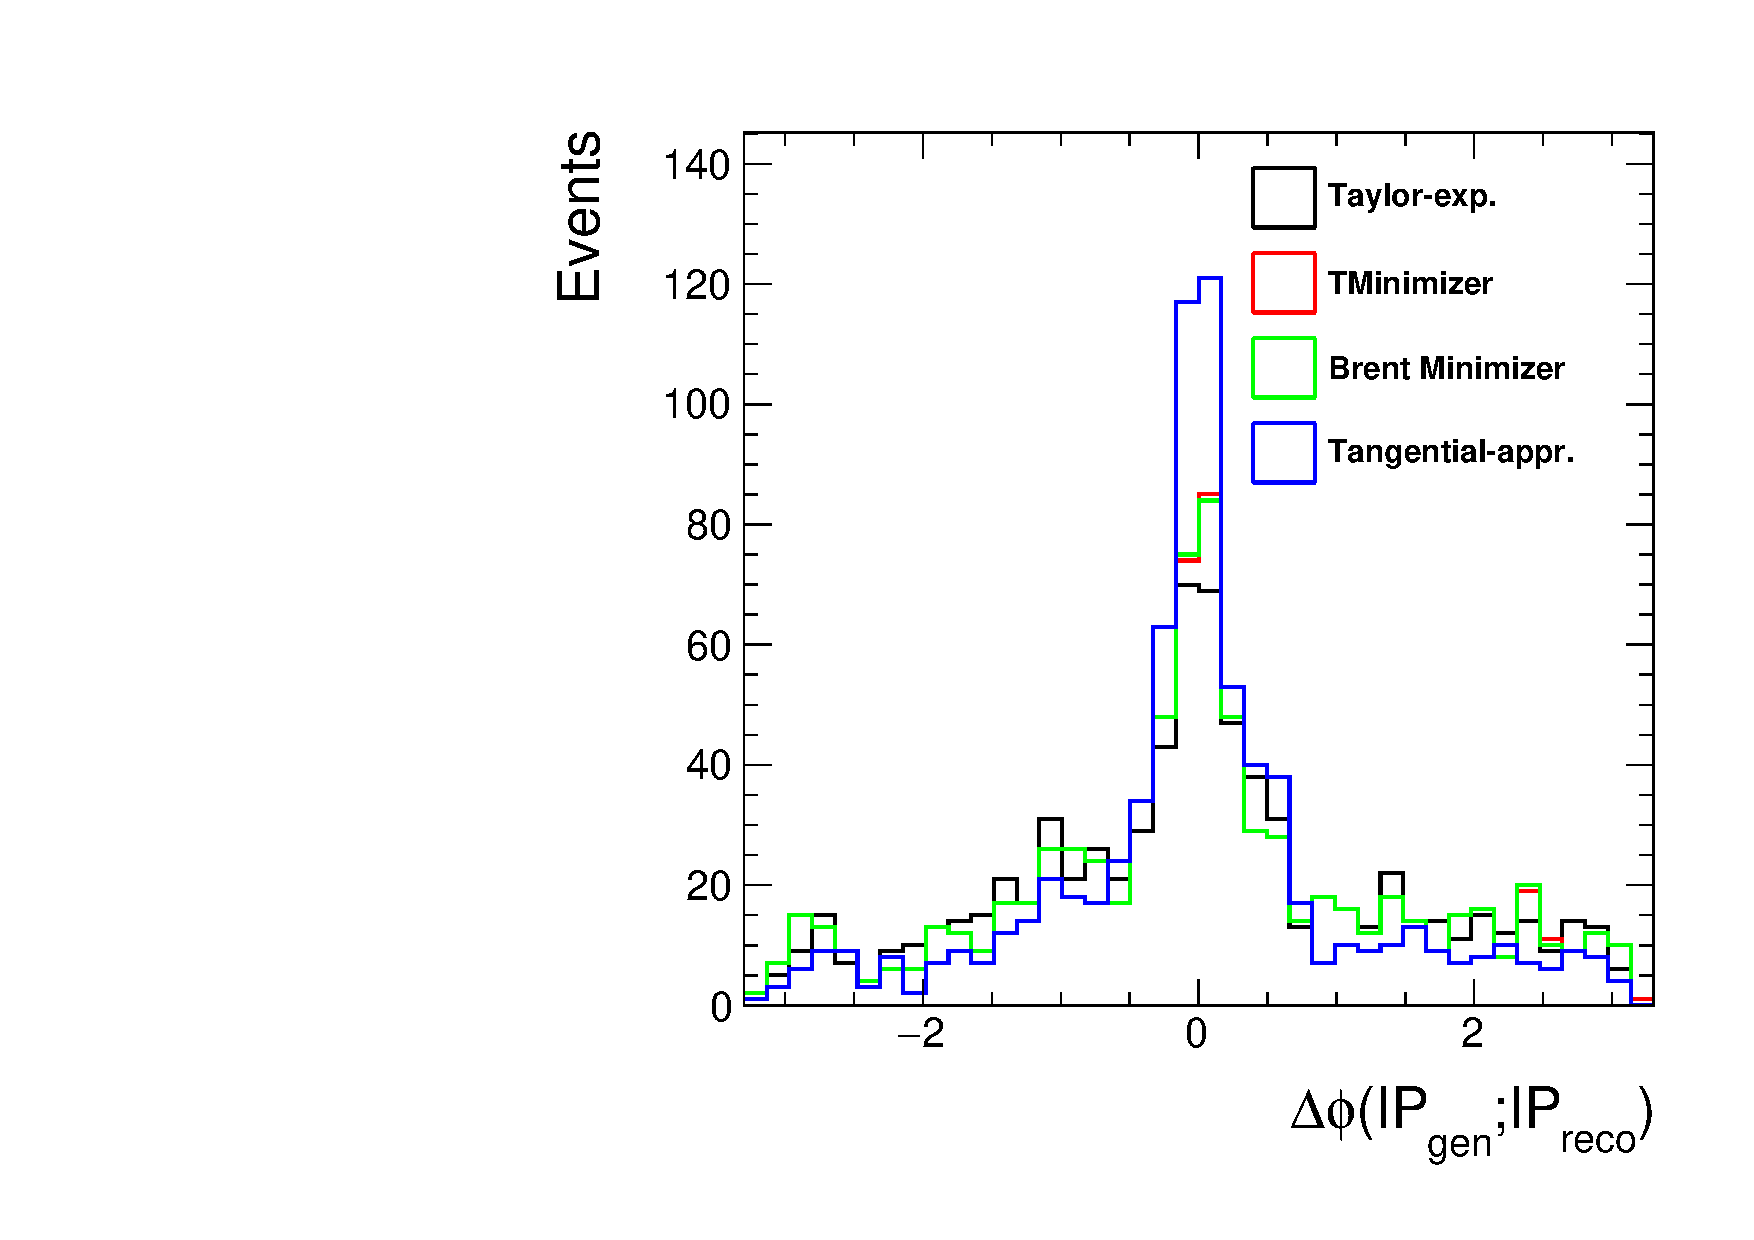
\includegraphics[width=0.7\linewidth]{Figures/deltaPhi_nocut}
	\caption{The comparison of generated and reconstructed IPs}
	\label{fig:deltaphinocut}
\end{figure}\\
For an algorithm performing better than the current tangential approximation, one expects a narrower distribution concerning $\Delta\phi$, since the data should deliver more reliable results. This is not the case however (no matter which numerical algorithm one considers meaning errors in the implementation can be excluded), which can be explained by the fact that the generated impact parameters are also calculated via the already discussed tangential approach.\\
While looking at these results, it is interesting to apply the cuts introduced in Chapter \ref{Chapter4}, which is portrayed in Fig. \ref{fig:deltaphicut}. Interestingly, a secondary peak arises around $\Delta\phi \approx -\pi/2$. This can be explained by the fact, that the primary vertex is not situated in the close neighbourhood of the origin, which can lead in some cases to systematic deviations in $\Delta\phi$.
\begin{figure}[h]
	\centering
	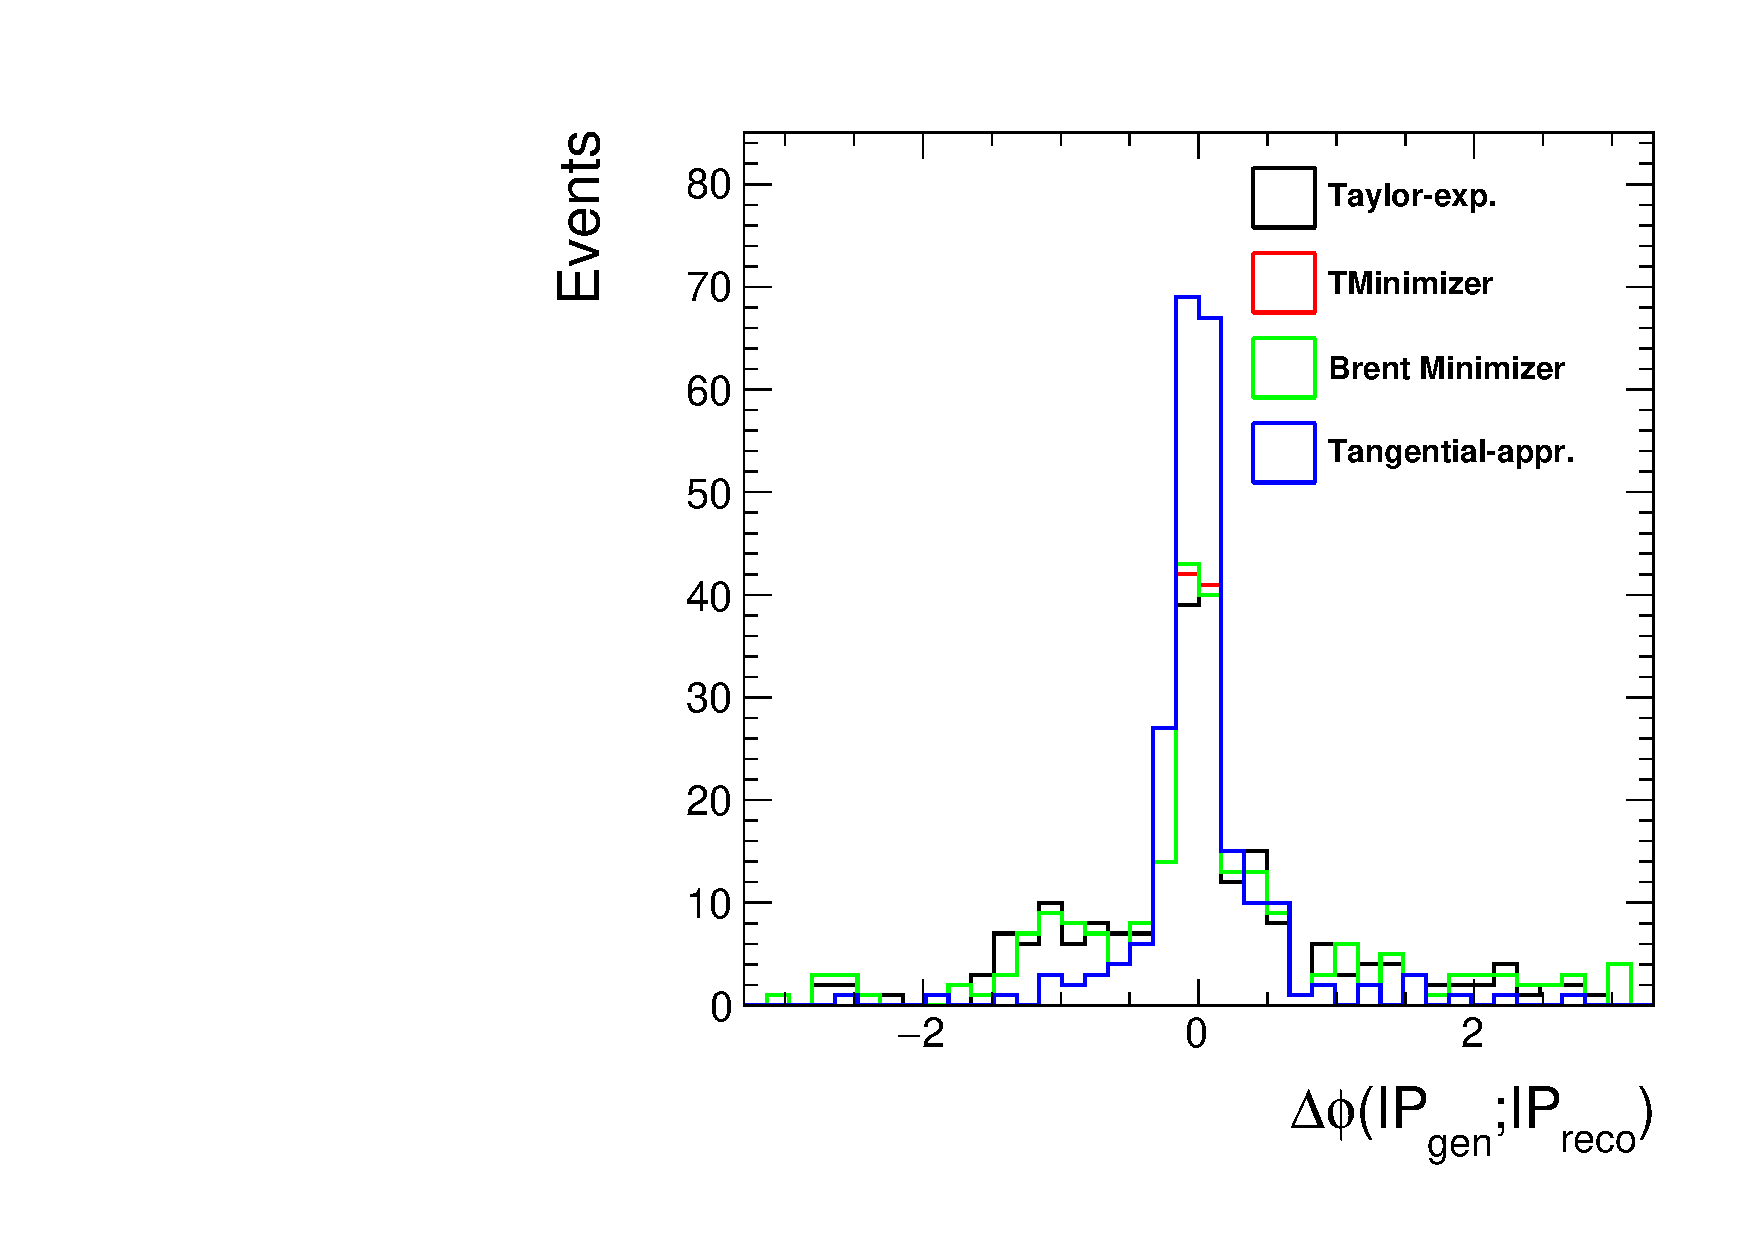
\includegraphics[width=0.7\linewidth]{Figures/deltaPhi_cut}
	\caption{The effect of cuts applied to the distribution of $\Delta\phi$. Here, only events with $d/\sigma_{\hat{d}} \geq 5$ were kept}
	\label{fig:deltaphicut}
\end{figure}

\subsection{Discussion of Validity}
In order to interpret and to see the validity of the helical approach, one has to take a look at the 2D geometry of the problem, shown in Fig. \ref{fig:geometry_diffIPs}, where $O$ corresponds to the origin of the coordinate system, \textbf{R} is the vector to the reference point (obtained from the track fit, being the closest point on the trajectory to $O$), $O'$ is the rotation centre of the helical trajectory and PV (SV) denote the primary (secondary) vertices respectively.
\begin{figure}[h]
	\centering
	\begin{tikzpicture}
	\centering
	
	\def\centerarc[#1](#2)(#3:#4:#5)% Syntax: [draw options] (center) (initial angle:final angle:radius)
	{ \draw[#1] ($(#2)+({#5*cos(#3)},{#5*sin(#3)})$) arc (#3:#4:#5); }
	
	\centerarc[<-](0,0)(60:90:8);
	\node[anchor = south] at ($({8*cos(60)},{8*sin(60)})$) {$l$};
	\centerarc[name path = h, dotted,line width=0.3mm, black](0,0)(90:160:8);
	\draw[densely dashed] (-5,8) --(5,8);
	\fill (0,0) circle (2pt) node[anchor=west] {O'};
	\draw[dashed] (0,0) --(0,8) node[anchor = east] at (0,4) {R};
	\fill (0,8) circle (1pt) node[anchor = south] {SV};
	\draw[line width=0.4mm,->] (0,8) -- (3,8) node[anchor=south east] {$p_T$};
	\draw[dashed,line width=0.4mm,->] (-3,5) -- (0,8) node[anchor = west] at (-1.5,6.5) {$\tau$};
	\draw[line width=0.6mm,->] (-3,5) -- (-3,8) node[anchor = west] at (-3,6.5) {$IP_{theo}$};
	\path [name path=OV] (-3,5) -- ++(-3,5);
	\draw [name intersections={of=OV and h, by=x}, ->] [very thick,blue] (-3,5) -- (x) node[below = 10pt] at (x) {$IP_{hel}$};
	\fill ($({6*cos(150)},{6*sin(150)})$) circle (2pt) node[anchor = north] {O};
	\draw[densely dashed, name path=tangent] ($({8*cos(150)},{8*sin(150)})$) --++($({8*sin(150)},{-8*cos(150)})$);
	\draw[dashed] ($({8*cos(150)},{8*sin(150)})$) -- ++ ($({-3*sin(150)},{3*cos(150)})$);
	\draw[line width=0.6mm,->] ($({6*cos(150)},{6*sin(150)})$)--($({8*cos(150)},{8*sin(150)})$)  node[anchor = east] {R};
	\path [name path = V_orth_to_tangent] (-3,5) --++($({6*cos(150)},{6*sin(150)})$);
	\draw [name intersections={of=V_orth_to_tangent and tangent, by=x}, ->] [very thick,red] (-3,5) -- (x) node[left = 1pt] at (x) {$IP_{tan}$};
	\fill (-3,5) circle (2pt) node[anchor=north] {PV};
	\end{tikzpicture}
	\caption{Visualisation of the IPs obtained by different algorithms in the 2D case.}
	\label{fig:geometry_diffIPs}
\end{figure}\\
In this graph, one can immediately see that in cases where the primary vertex is far from the origin $O$, the tangential approach becomes meaningless. In addition, one can see the extreme effect of displacement of the IP-vector due to the introduction of the reference point $R$, the angle between the theoretical and the reconstructed IP having approximately doubled. Let alone this would be enough reason to omit the previous approach and to look for an alternative.\\
On the other hand, the fact of ignoring the arbitrarily introduced point \textbf{R} should deliver better results, which would have manifested in a narrower distribution. Nevertheless, each IP-vector on generator level have also been calculated with the tangential approach, meaning the "true" impact parameters on generator level are missing. For this reason, a further comparison of this method with the "exact" IPs is necessary.\\
The root of the problem lies within the fact, that the $\tau$-particles coming from primary vertex cannot be fully reconstructed, or equivalently, the secondary vertex can only be reconstructed at the cost of great uncertainties. For this reason, one could also execute a kinematical fit with respect to the $\tau$ leptons in order to determine the location of the SV, from which, by minimizing the distance between the PV and the tangent defined by the 3-momentum of $l$, the correct IP-vector can be obtained. However, this goes beyond the scope of this thesis.
% Chapter Help

\chapter{Conclusion and Outlook} % Main chapter title

\label{Chapter6} % For referencing the chapter elsewhere, use \ref{Chapter1} 


TODO:
\begin{itemize}
	\item Influence of detector upgrades
\end{itemize}
\label{sec:conclusion}

%% Chapter Help

\chapter{Help and How-To-s} % Main chapter title

\label{Chapter_help} % For referencing the chapter elsewhere, use \ref{Chapter1} 

%----------------------------------------------------------------------------------------

% Define some commands to keep the formatting separated from the content 
\newcommand{\keyword}[1]{\textbf{#1}}
\newcommand{\tabhead}[1]{\textbf{#1}}
\newcommand{\code}[1]{\texttt{#1}}
\newcommand{\file}[1]{\texttt{\bfseries#1}}
\newcommand{\option}[1]{\texttt{\itshape#1}}

%----------------------------------------------------------------------------------------

\section{Welcome and Thank You}
Welcome to this \LaTeX{} Thesis Template, a beautiful and easy to use template for writing a thesis using the \LaTeX{} typesetting system.

If you are writing a thesis (or will be in the future) and its subject is technical or mathematical (though it doesn't have to be), then creating it in \LaTeX{} is highly recommended as a way to make sure you can just get down to the essential writing without having to worry over formatting or wasting time arguing with your word processor.

\LaTeX{} is easily able to professionally typeset documents that run to hundreds or thousands of pages long. With simple mark-up commands, it automatically sets out the table of contents, margins, page headers and footers and keeps the formatting consistent and beautiful. One of its main strengths is the way it can easily typeset mathematics, even \emph{heavy} mathematics. Even if those equations are the most horribly twisted and most difficult mathematical problems that can only be solved on a super-computer, you can at least count on \LaTeX{} to make them look stunning.

%----------------------------------------------------------------------------------------

\section{Learning \LaTeX{}}

\LaTeX{} is not a \textsc{wysiwyg} (What You See is What You Get) program, unlike word processors such as Microsoft Word or Apple's Pages. Instead, a document written for \LaTeX{} is actually a simple, plain text file that contains \emph{no formatting}. You tell \LaTeX{} how you want the formatting in the finished document by writing in simple commands amongst the text, for example, if I want to use \emph{italic text for emphasis}, I write the \verb|\emph{text}| command and put the text I want in italics in between the curly braces. This means that \LaTeX{} is a \enquote{mark-up} language, very much like HTML.

\subsection{A (not so short) Introduction to \LaTeX{}}

If you are new to \LaTeX{}, there is a very good eBook -- freely available online as a PDF file -- called, \enquote{The Not So Short Introduction to \LaTeX{}}. The book's title is typically shortened to just \emph{lshort}. You can download the latest version (as it is occasionally updated) from here:
\url{http://www.ctan.org/tex-archive/info/lshort/english/lshort.pdf}

It is also available in several other languages. Find yours from the list on this page: \url{http://www.ctan.org/tex-archive/info/lshort/}

It is recommended to take a little time out to learn how to use \LaTeX{} by creating several, small `test' documents, or having a close look at several templates on:\\ 
\url{http://www.LaTeXTemplates.com}\\ 
Making the effort now means you're not stuck learning the system when what you \emph{really} need to be doing is writing your thesis.

\subsection{A Short Math Guide for \LaTeX{}}

If you are writing a technical or mathematical thesis, then you may want to read the document by the AMS (American Mathematical Society) called, \enquote{A Short Math Guide for \LaTeX{}}. It can be found online here:
\url{http://www.ams.org/tex/amslatex.html}
under the \enquote{Additional Documentation} section towards the bottom of the page.

\subsection{Common \LaTeX{} Math Symbols}
There are a multitude of mathematical symbols available for \LaTeX{} and it would take a great effort to learn the commands for them all. The most common ones you are likely to use are shown on this page:
\url{http://www.sunilpatel.co.uk/latex-type/latex-math-symbols/}

You can use this page as a reference or crib sheet, the symbols are rendered as large, high quality images so you can quickly find the \LaTeX{} command for the symbol you need.

\subsection{\LaTeX{} on a Mac}
 
The \LaTeX{} distribution is available for many systems including Windows, Linux and Mac OS X. The package for OS X is called MacTeX and it contains all the applications you need -- bundled together and pre-customized -- for a fully working \LaTeX{} environment and work flow.
 
MacTeX includes a custom dedicated \LaTeX{} editor called TeXShop for writing your `\file{.tex}' files and BibDesk: a program to manage your references and create your bibliography section just as easily as managing songs and creating playlists in iTunes.

%----------------------------------------------------------------------------------------

\section{Getting Started with this Template}

If you are familiar with \LaTeX{}, then you should explore the directory structure of the template and then proceed to place your own information into the \emph{THESIS INFORMATION} block of the \file{main.tex} file. You can then modify the rest of this file to your unique specifications based on your degree/university. Section \ref{FillingFile} on page \pageref{FillingFile} will help you do this. Make sure you also read section \ref{ThesisConventions} about thesis conventions to get the most out of this template.

If you are new to \LaTeX{} it is recommended that you carry on reading through the rest of the information in this document.

Before you begin using this template you should ensure that its style complies with the thesis style guidelines imposed by your institution. In most cases this template style and layout will be suitable. If it is not, it may only require a small change to bring the template in line with your institution's recommendations. These modifications will need to be done on the \file{MastersDoctoralThesis.cls} file.

\subsection{About this Template}

This \LaTeX{} Thesis Template is originally based and created around a \LaTeX{} style file created by Steve R.\ Gunn from the University of Southampton (UK), department of Electronics and Computer Science. You can find his original thesis style file at his site, here:
\url{http://www.ecs.soton.ac.uk/~srg/softwaretools/document/templates/}

Steve's \file{ecsthesis.cls} was then taken by Sunil Patel who modified it by creating a skeleton framework and folder structure to place the thesis files in. The resulting template can be found on Sunil's site here:
\url{http://www.sunilpatel.co.uk/thesis-template}

Sunil's template was made available through \url{http://www.LaTeXTemplates.com} where it was modified many times based on user requests and questions. Version 2.0 and onwards of this template represents a major modification to Sunil's template and is, in fact, hardly recognisable. The work to make version 2.0 possible was carried out by \href{mailto:vel@latextemplates.com}{Vel} and Johannes Böttcher.

%----------------------------------------------------------------------------------------

\section{What this Template Includes}

\subsection{Folders}

This template comes as a single zip file that expands out to several files and folders. The folder names are mostly self-explanatory:

\keyword{Appendices} -- this is the folder where you put the appendices. Each appendix should go into its own separate \file{.tex} file. An example and template are included in the directory.

\keyword{Chapters} -- this is the folder where you put the thesis chapters. A thesis usually has about six chapters, though there is no hard rule on this. Each chapter should go in its own separate \file{.tex} file and they can be split as:
\begin{itemize}
\item Chapter 1: Introduction to the thesis topic
\item Chapter 2: Background information and theory
\item Chapter 3: (Laboratory) experimental setup
\item Chapter 4: Details of experiment 1
\item Chapter 5: Details of experiment 2
\item Chapter 6: Discussion of the experimental results
\item Chapter 7: Conclusion and future directions
\end{itemize}
This chapter layout is specialised for the experimental sciences, your discipline may be different.

\keyword{Figures} -- this folder contains all figures for the thesis. These are the final images that will go into the thesis document.

\subsection{Files}

Included are also several files, most of them are plain text and you can see their contents in a text editor. After initial compilation, you will see that more auxiliary files are created by \LaTeX{} or BibTeX and which you don't need to delete or worry about:

\keyword{example.bib} -- this is an important file that contains all the bibliographic information and references that you will be citing in the thesis for use with BibTeX. You can write it manually, but there are reference manager programs available that will create and manage it for you. Bibliographies in \LaTeX{} are a large subject and you may need to read about BibTeX before starting with this. Many modern reference managers will allow you to export your references in BibTeX format which greatly eases the amount of work you have to do.

\keyword{MastersDoctoralThesis.cls} -- this is an important file. It is the class file that tells \LaTeX{} how to format the thesis. 

\keyword{main.pdf} -- this is your beautifully typeset thesis (in the PDF file format) created by \LaTeX{}. It is supplied in the PDF with the template and after you compile the template you should get an identical version.

\keyword{main.tex} -- this is an important file. This is the file that you tell \LaTeX{} to compile to produce your thesis as a PDF file. It contains the framework and constructs that tell \LaTeX{} how to layout the thesis. It is heavily commented so you can read exactly what each line of code does and why it is there. After you put your own information into the \emph{THESIS INFORMATION} block -- you have now started your thesis!

Files that are \emph{not} included, but are created by \LaTeX{} as auxiliary files include:

\keyword{main.aux} -- this is an auxiliary file generated by \LaTeX{}, if it is deleted \LaTeX{} simply regenerates it when you run the main \file{.tex} file.

\keyword{main.bbl} -- this is an auxiliary file generated by BibTeX, if it is deleted, BibTeX simply regenerates it when you run the \file{main.aux} file. Whereas the \file{.bib} file contains all the references you have, this \file{.bbl} file contains the references you have actually cited in the thesis and is used to build the bibliography section of the thesis.

\keyword{main.blg} -- this is an auxiliary file generated by BibTeX, if it is deleted BibTeX simply regenerates it when you run the main \file{.aux} file.

\keyword{main.lof} -- this is an auxiliary file generated by \LaTeX{}, if it is deleted \LaTeX{} simply regenerates it when you run the main \file{.tex} file. It tells \LaTeX{} how to build the \emph{List of Figures} section.

\keyword{main.log} -- this is an auxiliary file generated by \LaTeX{}, if it is deleted \LaTeX{} simply regenerates it when you run the main \file{.tex} file. It contains messages from \LaTeX{}, if you receive errors and warnings from \LaTeX{}, they will be in this \file{.log} file.

\keyword{main.lot} -- this is an auxiliary file generated by \LaTeX{}, if it is deleted \LaTeX{} simply regenerates it when you run the main \file{.tex} file. It tells \LaTeX{} how to build the \emph{List of Tables} section.

\keyword{main.out} -- this is an auxiliary file generated by \LaTeX{}, if it is deleted \LaTeX{} simply regenerates it when you run the main \file{.tex} file.

So from this long list, only the files with the \file{.bib}, \file{.cls} and \file{.tex} extensions are the most important ones. The other auxiliary files can be ignored or deleted as \LaTeX{} and BibTeX will regenerate them.

%----------------------------------------------------------------------------------------

\section{Filling in Your Information in the \file{main.tex} File}\label{FillingFile}

You will need to personalise the thesis template and make it your own by filling in your own information. This is done by editing the \file{main.tex} file in a text editor or your favourite LaTeX environment.

Open the file and scroll down to the third large block titled \emph{THESIS INFORMATION} where you can see the entries for \emph{University Name}, \emph{Department Name}, etc \ldots

Fill out the information about yourself, your group and institution. You can also insert web links, if you do, make sure you use the full URL, including the \code{http://} for this. If you don't want these to be linked, simply remove the \verb|\href{url}{name}| and only leave the name.

When you have done this, save the file and recompile \code{main.tex}. All the information you filled in should now be in the PDF, complete with web links. You can now begin your thesis proper!

%----------------------------------------------------------------------------------------

\section{The \code{main.tex} File Explained}

The \file{main.tex} file contains the structure of the thesis. There are plenty of written comments that explain what pages, sections and formatting the \LaTeX{} code is creating. Each major document element is divided into commented blocks with titles in all capitals to make it obvious what the following bit of code is doing. Initially there seems to be a lot of \LaTeX{} code, but this is all formatting, and it has all been taken care of so you don't have to do it.

Begin by checking that your information on the title page is correct. For the thesis declaration, your institution may insist on something different than the text given. If this is the case, just replace what you see with what is required in the \emph{DECLARATION PAGE} block.

Then comes a page which contains a funny quote. You can put your own, or quote your favourite scientist, author, person, and so on. Make sure to put the name of the person who you took the quote from.

Following this is the abstract page which summarises your work in a condensed way and can almost be used as a standalone document to describe what you have done. The text you write will cause the heading to move up so don't worry about running out of space.

Next come the acknowledgements. On this page, write about all the people who you wish to thank (not forgetting parents, partners and your advisor/supervisor).

The contents pages, list of figures and tables are all taken care of for you and do not need to be manually created or edited. The next set of pages are more likely to be optional and can be deleted since they are for a more technical thesis: insert a list of abbreviations you have used in the thesis, then a list of the physical constants and numbers you refer to and finally, a list of mathematical symbols used in any formulae. Making the effort to fill these tables means the reader has a one-stop place to refer to instead of searching the internet and references to try and find out what you meant by certain abbreviations or symbols.

The list of symbols is split into the Roman and Greek alphabets. Whereas the abbreviations and symbols ought to be listed in alphabetical order (and this is \emph{not} done automatically for you) the list of physical constants should be grouped into similar themes.

The next page contains a one line dedication. Who will you dedicate your thesis to?

Finally, there is the block where the chapters are included. Uncomment the lines (delete the \code{\%} character) as you write the chapters. Each chapter should be written in its own file and put into the \emph{Chapters} folder and named \file{Chapter1}, \file{Chapter2}, etc\ldots Similarly for the appendices, uncomment the lines as you need them. Each appendix should go into its own file and placed in the \emph{Appendices} folder.

After the preamble, chapters and appendices finally comes the bibliography. The bibliography style (called \option{authoryear}) is used for the bibliography and is a fully featured style that will even include links to where the referenced paper can be found online. Do not underestimate how grateful your reader will be to find that a reference to a paper is just a click away. Of course, this relies on you putting the URL information into the BibTeX file in the first place.

%----------------------------------------------------------------------------------------

\section{Thesis Features and Conventions}\label{ThesisConventions}

To get the best out of this template, there are a few conventions that you may want to follow.

One of the most important (and most difficult) things to keep track of in such a long document as a thesis is consistency. Using certain conventions and ways of doing things (such as using a Todo list) makes the job easier. Of course, all of these are optional and you can adopt your own method.

\subsection{Printing Format}

This thesis template is designed for double sided printing (i.e. content on the front and back of pages) as most theses are printed and bound this way. Switching to one sided printing is as simple as uncommenting the \option{oneside} option of the \code{documentclass} command at the top of the \file{main.tex} file. You may then wish to adjust the margins to suit specifications from your institution.

The headers for the pages contain the page number on the outer side (so it is easy to flick through to the page you want) and the chapter name on the inner side.

The text is set to 11 point by default with single line spacing, again, you can tune the text size and spacing should you want or need to using the options at the very start of \file{main.tex}. The spacing can be changed similarly by replacing the \option{singlespacing} with \option{onehalfspacing} or \option{doublespacing}.

\subsection{Using US Letter Paper}

The paper size used in the template is A4, which is the standard size in Europe. If you are using this thesis template elsewhere and particularly in the United States, then you may have to change the A4 paper size to the US Letter size. This can be done in the margins settings section in \file{main.tex}.

Due to the differences in the paper size, the resulting margins may be different to what you like or require (as it is common for institutions to dictate certain margin sizes). If this is the case, then the margin sizes can be tweaked by modifying the values in the same block as where you set the paper size. Now your document should be set up for US Letter paper size with suitable margins.

\subsection{References}

The \code{biblatex} package is used to format the bibliography and inserts references such as this one \parencite{Reference1}. The options used in the \file{main.tex} file mean that the in-text citations of references are formatted with the author(s) listed with the date of the publication. Multiple references are separated by semicolons (e.g. \parencite{Reference2, Reference1}) and references with more than three authors only show the first author with \emph{et al.} indicating there are more authors (e.g. \parencite{Reference3}). This is done automatically for you. To see how you use references, have a look at the \file{Chapter1.tex} source file. Many reference managers allow you to simply drag the reference into the document as you type.

Scientific references should come \emph{before} the punctuation mark if there is one (such as a comma or period). The same goes for footnotes\footnote{Such as this footnote, here down at the bottom of the page.}. You can change this but the most important thing is to keep the convention consistent throughout the thesis. Footnotes themselves should be full, descriptive sentences (beginning with a capital letter and ending with a full stop). The APA6 states: \enquote{Footnote numbers should be superscripted, [...], following any punctuation mark except a dash.} The Chicago manual of style states: \enquote{A note number should be placed at the end of a sentence or clause. The number follows any punctuation mark except the dash, which it precedes. It follows a closing parenthesis.}

The bibliography is typeset with references listed in alphabetical order by the first author's last name. This is similar to the APA referencing style. To see how \LaTeX{} typesets the bibliography, have a look at the very end of this document (or just click on the reference number links in in-text citations).

\subsubsection{A Note on bibtex}

The bibtex backend used in the template by default does not correctly handle unicode character encoding (i.e. "international" characters). You may see a warning about this in the compilation log and, if your references contain unicode characters, they may not show up correctly or at all. The solution to this is to use the biber backend instead of the outdated bibtex backend. This is done by finding this in \file{main.tex}: \option{backend=bibtex} and changing it to \option{backend=biber}. You will then need to delete all auxiliary BibTeX files and navigate to the template directory in your terminal (command prompt). Once there, simply type \code{biber main} and biber will compile your bibliography. You can then compile \file{main.tex} as normal and your bibliography will be updated. An alternative is to set up your LaTeX editor to compile with biber instead of bibtex, see \href{http://tex.stackexchange.com/questions/154751/biblatex-with-biber-configuring-my-editor-to-avoid-undefined-citations/}{here} for how to do this for various editors.

\subsection{Tables}

Tables are an important way of displaying your results, below is an example table which was generated with this code:

{\small
\begin{verbatim}
\begin{table}
\caption{The effects of treatments X and Y on the four groups studied.}
\label{tab:treatments}
\centering
\begin{tabular}{l l l}
\toprule
\tabhead{Groups} & \tabhead{Treatment X} & \tabhead{Treatment Y} \\
\midrule
1 & 0.2 & 0.8\\
2 & 0.17 & 0.7\\
3 & 0.24 & 0.75\\
4 & 0.68 & 0.3\\
\bottomrule\\
\end{tabular}
\end{table}
\end{verbatim}
}

\begin{table}
\caption{The effects of treatments X and Y on the four groups studied.}
\label{tab:treatments}
\centering
\begin{tabular}{l l l}
\toprule
\tabhead{Groups} & \tabhead{Treatment X} & \tabhead{Treatment Y} \\
\midrule
1 & 0.2 & 0.8\\
2 & 0.17 & 0.7\\
3 & 0.24 & 0.75\\
4 & 0.68 & 0.3\\
\bottomrule\\
\end{tabular}
\end{table}

You can reference tables with \verb|\ref{<label>}| where the label is defined within the table environment. See \file{Chapter1.tex} for an example of the label and citation (e.g. Table~\ref{tab:treatments}).

\subsection{Figures}

There will hopefully be many figures in your thesis (that should be placed in the \emph{Figures} folder). The way to insert figures into your thesis is to use a code template like this:
\begin{verbatim}
\begin{figure}
\centering

\includegraphics{Figures/Electron}
\decoRule
\caption[An Electron]{An electron (artist's impression).}
\label{fig:Electron}
\end{figure}
\end{verbatim}
Also look in the source file. Putting this code into the source file produces the picture of the electron that you can see in the figure below.

\begin{figure}[th]
\centering

\includegraphics{Figures/Electron}
\decoRule
\caption[An Electron]{An electron (artist's impression).}
\label{fig:Electron}
\end{figure}

Sometimes figures don't always appear where you write them in the source. The placement depends on how much space there is on the page for the figure. Sometimes there is not enough room to fit a figure directly where it should go (in relation to the text) and so \LaTeX{} puts it at the top of the next page. Positioning figures is the job of \LaTeX{} and so you should only worry about making them look good!

Figures usually should have captions just in case you need to refer to them (such as in Figure~\ref{fig:Electron}). The \verb|\caption| command contains two parts, the first part, inside the square brackets is the title that will appear in the \emph{List of Figures}, and so should be short. The second part in the curly brackets should contain the longer and more descriptive caption text.

The \verb|\decoRule| command is optional and simply puts an aesthetic horizontal line below the image. If you do this for one image, do it for all of them.

\LaTeX{} is capable of using images in pdf, jpg and png format.

\subsection{Typesetting mathematics}

If your thesis is going to contain heavy mathematical content, be sure that \LaTeX{} will make it look beautiful, even though it won't be able to solve the equations for you.

The \enquote{Not So Short Introduction to \LaTeX} (available on \href{http://www.ctan.org/tex-archive/info/lshort/english/lshort.pdf}{CTAN}) should tell you everything you need to know for most cases of typesetting mathematics. If you need more information, a much more thorough mathematical guide is available from the AMS called, \enquote{A Short Math Guide to \LaTeX} and can be downloaded from:
\url{ftp://ftp.ams.org/pub/tex/doc/amsmath/short-math-guide.pdf}

There are many different \LaTeX{} symbols to remember, luckily you can find the most common symbols in \href{http://ctan.org/pkg/comprehensive}{The Comprehensive \LaTeX~Symbol List}.

You can write an equation, which is automatically given an equation number by \LaTeX{} like this:
\begin{verbatim}
\begin{equation}
E = mc^{2}
\label{eqn:Einstein}
\end{equation}
\end{verbatim}

This will produce Einstein's famous energy-matter equivalence equation:
\begin{equation}
E = mc^{2}
\label{eqn:Einstein}
\end{equation}

All equations you write (which are not in the middle of paragraph text) are automatically given equation numbers by \LaTeX{}. If you don't want a particular equation numbered, use the unnumbered form:
\begin{verbatim}
\[ a^{2}=4 \]
\end{verbatim}

%----------------------------------------------------------------------------------------

\section{Sectioning and Subsectioning}

You should break your thesis up into nice, bite-sized sections and subsections. \LaTeX{} automatically builds a table of Contents by looking at all the \verb|\chapter{}|, \verb|\section{}|  and \verb|\subsection{}| commands you write in the source.

The Table of Contents should only list the sections to three (3) levels. A \verb|chapter{}| is level zero (0). A \verb|\section{}| is level one (1) and so a \verb|\subsection{}| is level two (2). In your thesis it is likely that you will even use a \verb|subsubsection{}|, which is level three (3). The depth to which the Table of Contents is formatted is set within \file{MastersDoctoralThesis.cls}. If you need this changed, you can do it in \file{main.tex}.

%----------------------------------------------------------------------------------------

\section{In Closing}

You have reached the end of this mini-guide. You can now rename or overwrite this pdf file and begin writing your own \file{Chapter1.tex} and the rest of your thesis. The easy work of setting up the structure and framework has been taken care of for you. It's now your job to fill it out!

Good luck and have lots of fun!

\begin{flushright}
Guide written by ---\\
Sunil Patel: \href{http://www.sunilpatel.co.uk}{www.sunilpatel.co.uk}\\
Vel: \href{http://www.LaTeXTemplates.com}{LaTeXTemplates.com}
\end{flushright}


%----------------------------------------------------------------------------------------
%	THESIS CONTENT - APPENDICES
%----------------------------------------------------------------------------------------

\appendix % Cue to tell LaTeX that the following "chapters" are Appendices

% Include the appendices of the thesis as separate files from the Appendices folder
% Uncomment the lines as you write the Appendices

% Appendix Template

\chapter{The Approximation of the Helix} % Main appendix title

\label{AppendixA}
Since most of the particles considered in this thesis are travelling at velocities close to the speed of light, one can assume that $\delta t = \omega \cdot t << 1$, such that one can approximate the helix via
\begin{multline}
	\boldsymbol{x}(t) = \boldsymbol{O'} +  \left(\begin{tabular}{c}
	$R\cos(\delta t + \varphi_1) $\\ 
	$-R\sin(\delta t + \varphi_1) $\\ 
	$v_z t $
	\end{tabular} \right) = \boldsymbol{R} +  \delta t \cdot \left(\begin{tabular}{c}
	$-R\sin(\varphi_1) $\\ 
	$-R\cos(\varphi_1) $\\ 
	$v_3$
	\end{tabular}\right) \\ +\frac{(\delta t)^2}{2} \cdot R \left(\begin{tabular}{c}
	$-\cos(\varphi_1) $\\ 
	$\sin(\varphi_1) $\\ 
	$0$
	\end{tabular}\right)+\frac{(\delta t)^3}{6} \cdot R \left(\begin{tabular}{c}
	$\sin(\varphi_1) $\\ 
	$\cos(\varphi_1) $\\ 
	$0$
	\end{tabular}\right)+O((\delta t)^4),
\end{multline}
with $v_3 \delta t = v_z t = v_z \frac{\delta t}{\omega}$ such that the minimization problem becomes
\begin{equation}
	\delta(t) = |\overrightarrow{OV}-\boldsymbol{x}(t)|^2 = |\underbrace{\overrightarrow{OV}-\boldsymbol{R}}_\text{$\boldsymbol{\Delta}$}-\boldsymbol{f}(\delta t)|^2 = |\boldsymbol{\Delta}-\boldsymbol{f}(\delta t)|^2,
\end{equation}
with $\overrightarrow{OV}$ denoting the vector to the primary vertex. One has to expand $\delta(t)$ up to third order in $\delta t$, in order to solve
\begin{equation}
	\frac{d\delta(t)}{d\delta t} \stackrel{!}{=} 0
\end{equation}
analytically, which yields
\begin{equation}
	\delta (t) = \boldsymbol{\Delta}^2 - 2 \cdot \boldsymbol{\Delta}\cdot\boldsymbol{f} + \boldsymbol{f}^2 = \boldsymbol{\Delta}^2- 2 \cdot \boldsymbol{\Delta}\cdot\boldsymbol{f}+(\delta t)^2 (R^2+v^2_3).
\end{equation}
After an algebraic calculation one obtains as condition
\begin{multline}
	(\delta t)^2 \underbrace{\left[-2\left(\Delta_x \frac{R}{2}\sin\varphi_1+ \Delta_y\frac{R}{2}\cos\varphi_1\right)\right]}_\text{A} + \\
	\delta t \underbrace{\left[-2(\Delta_x R\cos\varphi_1 + \Delta_y R \sin\varphi_1)+2(R^2+v^2_3)\right]}_\text{B} + \\
	\underbrace{-2 \left[-\Delta_x R \sin\varphi_1-\Delta_y R \cos\varphi_1+\Delta_z v_3\right]}_\text{C}=0,
\end{multline}
leading to an ordinary secondary equation in $\delta t$, which can be solved analytically.
%\include{Appendices/AppendixB}
%\include{Appendices/AppendixC}

%----------------------------------------------------------------------------------------
%	BIBLIOGRAPHY
%----------------------------------------------------------------------------------------

\printbibliography[heading=bibintoc]

%----------------------------------------------------------------------------------------

\end{document}  
